% \documentclass[12pt]{article}
\usepackage[left=0.25cm,top=1cm,right=0.25cm,bottom=1cm]{geometry}
\textwidth = 20cm
\hoffset = -1cm
\usepackage[utf8]{inputenc}
\usepackage[spanish,es-tabla]{babel}
\usepackage[autostyle,spanish=mexican]{csquotes}
\usepackage[tbtags]{amsmath}
\usepackage{nccmath}
\usepackage{amsthm}
\usepackage{amssymb}
\usepackage{graphicx}
\usepackage{standalone}
\usepackage[outdir=./]{epstopdf}
\usepackage{siunitx}
\usepackage{physics}
\usepackage{color}
\usepackage{float}
\usepackage{multicol}
%\usepackage{milista}
\usepackage{enumitem}
\usepackage{anyfontsize}
\usepackage{anysize}
\usepackage{enumitem}
\usepackage{capt-of}
\usepackage{bm}
\usepackage{relsize}
\usepackage{placeins}
\usepackage{empheq}
\usepackage{cancel}
\usepackage{wrapfig}
\spanishdecimal{.}
\renewcommand{\baselinestretch}{1.5} 
\renewcommand\labelenumii{\theenumi.{\arabic{enumii}}}
\newcommand{\ptilde}[1]{\ensuremath{{#1}^{\prime}}}
\newcommand{\stilde}[1]{\ensuremath{{#1}^{\prime \prime}}}
\newcommand{\ttilde}[1]{\ensuremath{{#1}^{\prime \prime \prime}}}
\newcommand{\ntilde}[2]{\ensuremath{{#1}^{(#2)}}}


% %\usepackage{showframe}
% \title{Transformadas de Fourier \\ \large {Tema 6 - Transformadas integrales} \vspace{-3ex}}
% \author{M. en C. Gustavo Contreras Mayén}
% \date{ }
% \begin{document}
% \vspace{-4cm}
% \maketitle
% \fontsize{14}{14}\selectfont
% \tableofcontents
% \newpage

\documentclass[12pt]{beamer}
\usepackage{../Estilos/BeamerMAF}
\usepackage[absolute, overlay]{textpos}
\usepackage{../Estilos/ColoresLatex}
\input{../Preambulos/preambulo_Beamer_Antibes_beaver}

\setbeamercolor{section in foot}{bg=amethyst, fg=white}
\setbeamercolor{subsection in foot}{bg=almond, fg=black}

\makeatletter
\setbeamertemplate{footline}
{
\leavevmode%
\hbox{%
\begin{beamercolorbox}[wd=.333333\paperwidth,ht=2.25ex,dp=1ex,center]{section in foot}%
  \usebeamerfont{section in foot} \insertsection
\end{beamercolorbox}%
\begin{beamercolorbox}[wd=.333333\paperwidth,ht=2.25ex,dp=1ex,center]{subsection in foot}%
  \usebeamerfont{subsection in foot}  \insertsubsection
\end{beamercolorbox}%
\begin{beamercolorbox}[wd=.333333\paperwidth,ht=2.25ex,dp=1ex,right]{date in head/foot}%
  \usebeamerfont{date in head/foot} \insertshortdate{} \hspace*{1.5em}
  \insertframenumber{} / \inserttotalframenumber \hspace*{2ex} 
\end{beamercolorbox}}%
\vskip0pt%
}
\makeatother
% \usefonttheme{serif}
\setbeamercolor{frametitle}{bg=champagne}
\resetcounteronoverlays{saveenumi}

\AtBeginDocument{\RenewCommandCopy\qty\SI}
\ExplSyntaxOn
\msg_redirect_name:nnn { siunitx } { physics-pkg } { none }
\ExplSyntaxOff

% \date{}

\title{\large{Tema 6 - Transformada de Fourier}}
\subtitle{Matemáticas Avanzadas de la Física}
\author{M. en C. Gustavo Contreras Mayén}
\date{\today}

\begin{document}
\maketitle
\fontsize{14}{14}\selectfont
\spanishdecimal{.}

\section*{Contenido}
\frame[allowframebreaks]{\frametitle{Contenido} \tableofcontents[currentsection, hideallsubsections]}


%Ref. Patra (2018) 1.2 Classes of functions.
% \section{Tipos de funciones.}

% Una función de valor único $f (x)$ de la variable independiente $x$ que es continua en un intervalo $[a, b]$, se dice que pertenece a una clase denotada por $f \in C \, [a, b]$.
% \par
% Se dice que una función $f (x)$ es continua por partes en un intervalo $(a, b)$ si el intervalo se puede dividir en un número finito de subintervalos que no se intersectan $(a, a_{1}), (a_{1}, a_{2}), \ldots, (a_{n -1}, b)$, en cada uno de los cuales la función es continua y tiene límites finitos cuando $x$ se acerca a los puntos extremos de cada uno de los subintervalos. Se dice que dicha función pertenece a una clase denotada por $f \in P \, (a, b)$.
% \par
% Una función continua a trozos $f$ en $(a, b)$, cuya derivada de primer orden es también una función continua a trozos en $(a, b)$ y pertenece a una clase denotada por $f \in P^{1} \, (a, b)$.
% \par
% Se dice que el conjunto de funciones $f (x)$ es absolutamente integrable sobre $\Omega$, si $\scaleint{6ex}_{\bs \Omega}  \abs{f (x)} \dd{x}$ es finito. Entonces decimos que esta función pertenece a una clase denotada por $f (x) \in A_{1} (\Omega)$. De manera similar, el hecho que $f \in A_{m} (\Omega)$ implica que $\scaleint{6ex}_{\bs \Omega}  \abs{f (x)} \dd{x}$ es finito.
% \par
% Finalmente, presentamos una clase de funciones $f (x)$, que satisface las siguientes condiciones:
% \begin{enumerate}[label=\roman*]
% \item $f (x)$ se define en $c < x < c + 2 \, l$.
% \item $f (x)$ es una función periódica del período $2 \, l$.
% \item $f (x)$ y $\pderivada{f} (x)$ son continuas por partes en $c  < x <c + 2 \, l$ expresado por $f (x) \in P^{1} (c, c + 2 \, l)$.
% \end{enumerate}
% Se dice que esta clase de función $f (x)$ satisface las condiciones de Dirichlet. Se dice que una función $f (x)$ es de orden exponencial $\sigma$ cuando $x \to \infty$, si las constantes $\sigma, m (> 0)$ se pueden encontrar de modo que:
% \begin{align*}
% \abs{ e^{\sigma \, x} \, f (x)} < m \hspace{1cm} \Longrightarrow \hspace{1cm} \abs{f (x)} < m \, e^{m \, \sigma} \hspace{0.5cm} x > x_{0}
% \end{align*}
% De manera equivalente, también se puede escribir $f (x) = 0 \, (e^{m \, \sigma})$ mientras $x \to \infty$.

% %Ref. Patra (2018) 1.3 Series de Fourier y la Fórmula Integral de Fourier.

% \section{Series de Fourier y la fórmula integral de Fourier.}

% Consideremos una función $f (x)$ que satisface las condiciones de Dirichlet en el intervalo $[-l, l]$, la función pertenece a la clase $P^{1} (R)$ y también a la clase $A_{1} (R)$. Sea el período principal de $f (x)$ igual a $2 \, l$. Entonces $f (x)$ admite una representación en una serie de Fourier:
% \begin{align*}
% f (x) = a_{0} + \nsum_{n=1}^{\infty} \left[ a_{n} \, \cos \left( \dfrac{n \, \pi, \, x}{l}  \right) + b_{n} \, \sin \left( \dfrac{n \, \pi, \, x}{l}  \right) \right]
% \end{align*}
% donde:
% \begin{align*}
% a_{0} &= \dfrac{1}{2 \, l} \scaleint{6ex}_{\bs -l}^{l} f (x) \dd{x} \\[0.5em]
% (a_{n}, b_{n}) &= \dfrac{1}{l} \scaleint{6ex}_{\bs -l}^{l} f (x) \left[ \cos \left( \dfrac{n \, \pi \, x}{l} \right), \sin \left( \dfrac{n \, \pi \, x}{l} \right) \right] \dd{x}
% \end{align*}
% entonces:
% \begin{align*}
% a_{n} - i \, b_{n} = \dfrac{1}{l} \scaleint{6ex}_{\bs -l}^{l} f (x) \, \exp \left( - \dfrac{i \, n \, \pi \, x}{l} \right) \dd{x}
% \end{align*}
% Definimos a continuación:
% \begin{align*}
% a_{0} &= c_{0} \\
% a_{n} &= c_{n} + c_{-n} \\
% i \, b_{n} &= c_{n} - c_{-n}
% \end{align*}
% Entonces tendremos que:
% \begin{align}
% \begin{aligned}[b]
% f (x) &= c_{0} + \nsum_{n=1}^{\infty} \left[ c_{n} \, \exp \left( -\dfrac{i \, n \, \pi \, x}{l} \right) + c_{-n} \, \exp \left( \dfrac{i \, n \, \pi \, x}{l} \right) \right] = \\[0.5em]
% &= \nsum_{-\infty}^{+\infty} c_{n} \, \exp \left( - \dfrac{i \, n \, \pi \, x}{l} \right)
% \end{aligned}
% \label{eq:ecuacion_01_02}
% \end{align}
% donde el coeficiente $c_{n}$ es:
% \begin{align}
% \begin{aligned}[b]
% c_{n} &= \dfrac{1}{2 \, l} \scaleint{6ex}_{\bs -l}^{l} f (x) \, \exp \left( \dfrac{i \, n \, \pi, x}{l} \right) \dd{x} = \\[0.5em]
% &= \dfrac{1}{2 \, l} \scaleint{6ex}_{\bs -l}^{l} f (t) \, \exp \left( \dfrac{i \, n \, \pi, t}{l} \right) \dd{t}
% \end{aligned}
% \label{eq:ecuacion_01_03}
% \end{align}
% Esta es forma de la serie de Fourier se le llama \emph{forma compleja de la serie de Fourier} en el intervalo $(-l , l)$.
% \par
% Por lo que de las ecs. (\ref{eq:ecuacion_01_02}) y (\ref{eq:ecuacion_01_03}), se obtiene:
% \begin{align}
% f (x) = \nsum_{-\infty}^{+\infty} \left[ \dfrac{1}{2 \, l} \scaleint{6ex}_{\bs -l}^{l} f (t) \exp \left( \dfrac{i \, n \, \pi \, t}{l} \right) \dd{t} \right] \, \exp \left( - \dfrac{i \, n \, \pi \, x}{l} \right)
% \label{eq:ecuacion_01_04}
% \end{align}
% Ahora hagamos el siguiente cambio de variable:
% \begin{align*}
% \dfrac{\pi}{l} = \delta \xi
% \end{align*}
% Notemos que $\delta \xi \to 0$ mientras $l \to \infty$, tal que $l \, \delta \xi = \pi =$ un número finito. Entonces la serie (\ref{eq:ecuacion_01_04}), antes de tomar el límite cuando $\delta \xi \to 0$, se convierte en:
% \begin{align*}
% f (x) &= \dfrac{1}{2 \, \pi} \nsum_{-\infty}^{+\infty} \delta \xi \, \left[ \scaleint{6ex}_{\bs -\frac{\pi}{\delta \xi}}^{\frac{\pi}{\delta \xi}} f (t) \, \exp \left( i \, n \, t \, \delta \xi \right) \dd{t} \right] \, \exp \left( - i \, n \, x \, \delta \xi \right) = \\[0.5em]
% &= \dfrac{1}{2 \, \pi} \scaleint{6ex}_{\bs -\frac{\pi}{\delta \xi}}^{\frac{\pi}{\delta \xi}} f (t) \, \left[ \nsum_{-\infty}^{+\infty} \delta \xi \, \exp \left( i \, n (t - x \, \delta \xi) \right) \right] \dd{t}
% \end{align*}
% después de intercambiar formalmente los signos de suma e integración. Dado que asumimos que  $f (x) \in P^{1} (R)$ y también que $f (x) \in A_{1} (R)$, haciendo que $\delta \xi \to 0$ y usando la definición de integral definida de Riemann como límite de una suma obtenemos:
% \begin{align}
% f (x) &= \dfrac{1}{2 \, \pi} \scaleint{6ex}_{\bs -\infty}^{\infty} f (t) \, \left[ \exp \left( i (t - x) \, y \right) \, \dd{y} \right] \dd{t} \label{eq:ecuacion_01_05} \\[0.5em]
% \Rightarrow f (x) &= \dfrac{1}{\sqrt{2 \, \pi}} \scaleint{6ex}_{\bs -\infty}^{\infty} \exp \left( i \, y \, x \right) \big[ F (y) \big] \dd{y} \label{eq:ecuacion_01_06} \\[0.5em]
% \mbox{donde} \hspace{0.5cm} F (y) &= \dfrac{1}{\sqrt{2 \, \pi}} \scaleint{6ex}_{\bs -\infty}^{\infty} f (t) \, \exp \left( i \, y \, t \right) \dd{t} \label{eq:ecuacion_01_07}
% \end{align}
% De nueva cuenta, de la ec. (\ref{eq:ecuacion_01_05}), se obtiene lo siguiente:
% \begin{align}
% f (x) = \dfrac{1}{\pi} \scaleint{6ex}_{\bs 0}^{\infty}  \dd{y} \, \scaleint{6ex}_{\bs -\infty}^{+\infty} f (t) \, \cos y (-t + x) \dd{t} \label{eq:ecuacion_01_08}
% \end{align}
% La ecuación (\ref{eq:ecuacion_01_08}) se le conoce como la \emph{fórmula integral de Fourier}.
% \par
% En un punto de discontinuidad finita de $f (x)$, el lado izquierdo de la ec. (\ref{eq:ecuacion_01_08}) se reemplaza con
% \begin{align*}
% \dfrac{1}{2} \big[ f (x + 0) + f (x - 0) \big]
% \end{align*}
% en el sentido de los valores límite.

%Referencia. Patra (2018) - An introduction to integral transforms. Sec. 1.4
\section{Las transformadas de Fourier}
\frame[allowframebreaks]{\frametitle{Temas a revisar} \tableofcontents[currentsection, hideothersubsections]}
\subsection{Definición}

\begin{frame}
\frametitle{Definiendo la transformada}
Una vez revisado el material introductorio, \pause podemos definir la \textocolor{ao}{transformada de Fourier} (TF) de una función continua por partes $f (x) \in P^{1} (R)$ y tal que $f (x) \in A_{1} (R)$.
\end{frame}
\begin{frame}
\frametitle{Definiendo la transformada}
La Transformada de Fourier (TF) se define por:
\pause
\begin{eqnarray}
\begin{aligned}[b]
&F \big[ f (x); x \to \xi \big] = \pause F \big[ f (x) \big] = \pause F (\xi) = \pause \overline{f} (\xi) = \\[0.5em] \pause
&= \dfrac{1}{\sqrt{2 \, \pi}} \scaleint{6ex}_{\bs -\infty}^{+\infty} f (x) \, \exp(i \, \xi \, x) \dd{x}
\end{aligned}
\label{eq:ecuacion_01_12}
\end{eqnarray}
\end{frame}
\begin{frame}
\frametitle{Definiendo la transformada}
Y también, la Transformada Inversa de Fourier (TIF):
\pause
\begin{eqnarray}
\begin{aligned}[b]
f (x) &= \pause F^{-1} \big[ F (\xi) \big] = \\[0.5em] \pause
&= \dfrac{1}{\sqrt{2 \, \pi}} \scaleint{6ex}_{\bs -\infty}^{+\infty} F (\xi) \, \exp(-i \, \xi \, x) \dd{\xi}
\label{eq:ecuacion_01_13}
\end{aligned}
\end{eqnarray}
en un punto continuo de $f (x)$.
\end{frame}
\begin{frame}
\frametitle{Definiendo la transformada}
\setbeamercolor{item projected}{bg=blue,fg=white}
\setbeamertemplate{enumerate items}{%
\usebeamercolor[bg]{item projected}%
\raisebox{1.5pt}{\colorbox{bg}{\color{fg}\footnotesize\insertenumlabel}}%
}
\begin{enumerate}[<+->]
\item La función $F (\xi)$ en la ec. (\ref{eq:ecuacion_01_12}) es la \textocolor{armygreen}{transformada de Fourier} de $f (x)$,
\item Mientras que $f (x)$ en la ec. (\ref{eq:ecuacion_01_13}) es la llamada \textocolor{red}{transformada inversa de Fourier} de $F (\xi)$.
\end{enumerate}
\end{frame}
\begin{frame}
\frametitle{Sobre la definición}
Algunos autores definen la transformada de Fourier  (ec. \ref{eq:ecuacion_01_12}) como:
\pause
\begin{eqnarray}
\begin{aligned}[b]
&F \big[ f (x); x \to \xi \big] = F (\xi) = \\[0.5em]
&= \scaleint{6ex}_{\bs -\infty}^{+\infty} f (x) \, \exp(i \, \xi \, x) \dd{x}
\label{eq:ecuacion_01_14}
\end{aligned}
\end{eqnarray}
\end{frame}
\begin{frame}
\frametitle{Sobre la definición}
Y la transformada inversa de Fourier (ec. \ref{eq:ecuacion_01_13}) como:
\pause
\begin{eqnarray}
f (x) = \dfrac{1}{2 \, \pi} \scaleint{6ex}_{\bs -\infty}^{+\infty} F (\xi) \, \exp(-i \, \xi \, x) \dd{\xi}
\label{eq:ecuacion_01_15}
\end{eqnarray}
\end{frame}
\begin{frame}
\frametitle{En puntos singulares}
En un punto de discontinuidad de $x \in R$, el lado izquierdo de las ecs. (\ref{eq:ecuacion_01_13}) y (\ref{eq:ecuacion_01_15}), toman la forma:
\pause
\begin{align*}
\dfrac{1}{2} \big[ f (x + 0) + f (x - 0) \big]
\end{align*}
en lugar de $f (x)$.
\end{frame}
\begin{frame}
\frametitle{Transformadas como operadores}
De las definiciones de las transformadas de Fourier y de la transformada inversa de Fourier, es posible escribir de la ec. (\ref{eq:ecuacion_01_12}):
\pause
\begin{eqnarray*}
\begin{aligned}
F (\xi) &= F \big[ f (x) \big] = F \big[ F^{-1} (F (\xi)) \big] \\[0.5em] \pause
&\Rightarrow \hspace{0.2cm} F \, F^{-1} \big[ F (\xi) \big] \equiv I \big[ F (\xi) \big] \\[0.5em] \pause
&\Rightarrow \hspace{0.2cm} F \, F^{-1} = I
\end{aligned}
\end{eqnarray*}
\end{frame}
\begin{frame}
\frametitle{Transformadas como operadores}
Que es un operador de identidad, entonces $F$ y $F^{-1}$ son los operadores de Fourier y su operador inverso respectivamente, y de la ec. (\ref{eq:ecuacion_01_13}):
\pause
\begin{eqnarray}
\begin{aligned}[b]
f (x) &= F^{-1} \big[ F (\xi) \big] = \pause F^{-1} \big[ F(f (x)) \big] = \\[0.5em] \pause 
&= F^{-1} \, F \big[ f (x) \big] \pause = I \big[ f (x) \big] \\[0.5em] \pause
&\Rightarrow \hspace{0.2cm} F^{-1} \, F = \pause I
\end{aligned}
\label{eq:ecuacion_01_16}
\end{eqnarray}
\end{frame}
\begin{frame}
\frametitle{Transformadas como operadores}    
Por lo que en una notación de operador:
\pause
\begin{align*}
F \, F^{-1} = F^{-1} \, F = I
\end{align*}
\pause
Esto demuestra que los operadores $F$ y $F^{-1}$ son conmutativos.
\end{frame}

\subsection{Transformadas Fourier seno y coseno}

\begin{frame}
\frametitle{Paridad de la función}
Consideremos que la función $f (x)$ sea una función \textocolor{armygreen}{impar} de $x \in R$, perteneciente además a las clases $P^{1} (R)$ y $A_{1} (R)$.
\\
\bigskip
\pause
Tenemos claramente que $f (-x) = - f (x)$. 
\end{frame}
\begin{frame}
\frametitle{La Transformada de Fourier seno}
De la ec. (\ref{eq:ecuacion_01_12}):
\pause
\begin{eqnarray}
\begin{aligned}[b]
&F \big[ f (x); x \to \xi \big] = \pause F (\xi) = \\[0.5em] \pause
&= \dfrac{1}{\sqrt{2 \, \pi}} \scaleint{6ex}_{\bs 0}^{\infty} f (x) \big[ \exp(i \xi x) {-} \exp(-i \xi x) \big] \dd{x} = \\[0.5em] \pause
&= i \, \sqrt{\dfrac{2}{\pi}} \scaleint{6ex}_{\bs 0}^{\infty} f (x) \, \sin \xi \, x \dd{x} = \\[0.5em] \pause
&\equiv i \, F_{s} (\xi)
\end{aligned}
\label{eq:ecuacion_01_17}
\end{eqnarray}
\end{frame}
\begin{frame}
\frametitle{La Transformada de Fourier seno}
Donde:
\pause
\begin{align}
F_{s} (\xi) = \sqrt{\dfrac{2}{\pi}} \scaleint{6ex}_{\bs 0}^{\infty} f (x) \, \sin \xi \, x \dd{x}
\label{eq:ecuacion_01_18}
\end{align}
La ec. (\ref{eq:ecuacion_01_18}) define la \textocolor{darkviolet}{transformada de Fourier seno} de la función $f (x)$.
\end{frame}
\begin{frame}
\frametitle{Relación entre transformadas}
Su conexión con la transformada de Fourier, está dada por la ec. (\ref{eq:ecuacion_01_17}) proporcionando $f (x)$ una función impar de $x \in R$.
\end{frame}
\begin{frame}
\frametitle{La Transformada de Fourier Inversa seno}
La expresión para la transformada inversa de (\ref{eq:ecuacion_01_18}) se define por:
\pause
\begin{align}
f (x) = \sqrt{\dfrac{2}{\pi}} \scaleint{6ex}_{\bs 0}^{\infty} F_{s}(\xi) \, \sin \xi \, x \dd{\xi}
\label{eq:ecuacion_01_19}
\end{align}
\end{frame}
\begin{frame}
\frametitle{La Transformada de Fourier coseno}
Sea ahora una función \textocolor{deepcarmine}{par} $f (x)$ de $x \in R$, \pause además de que pertenece a la clases $P^{1}(R)$ y $A_{1}(R)$.
\end{frame}
\begin{frame}
\frametitle{La Transformada de Fourier coseno}
Entonces: $f (-x) = f (x)$, por la ec. (\ref{eq:ecuacion_01_12}):
\pause
\begin{eqnarray}
\begin{aligned}[b]
&F \big[ f (x); x \to \xi \big] = F (\xi) = \\[0.5em] \pause
&= \dfrac{1}{\sqrt{2 \, \pi}} \scaleint{6ex}_{\bs 0}^{\infty} f (x) \big[ \exp(i \xi x) {+} \exp(-i \xi x) \big] \dd{x} = \\[0.5em] \pause
&= i \, \sqrt{\dfrac{2}{\pi}} \scaleint{6ex}_{\bs 0}^{\infty} f (x) \, \cos \xi \, x \dd{x} = \\[0.5em] \pause
&\equiv i \, F_{c} (\xi)    
\end{aligned}
\label{eq:ecuacion_01_20}
\end{eqnarray}
\end{frame}
\begin{frame}
\frametitle{La Transformada de Fourier coseno}
Donde:
\pause
\begin{align}
F_{c} (\xi) = \sqrt{\dfrac{2}{\pi}} \scaleint{6ex}_{\bs 0}^{\infty} f (x) \, \cos \xi \, x \dd{x}
\label{eq:ecuacion_01_21}
\end{align}
La ec. (\ref{eq:ecuacion_01_21}) define la \textocolor{denim}{transformada de Fourier coseno} de la función $f (x)$.
\end{frame}
\begin{frame}
\frametitle{Relación entre transformadas}
Su conexión con la transformada de Fourier, está dada por la ec. (\ref{eq:ecuacion_01_20}) proporcionando $f (x)$ una función par de $x \in R$.
\end{frame}
\begin{frame}
\frametitle{La Transformada de Fourier Inversa coseno}
La expresión para la transformada inversa de (\ref{eq:ecuacion_01_21}) se define por:
\pause
\begin{align}
f (x) = \sqrt{\dfrac{2}{\pi}} \scaleint{6ex}_{\bs 0}^{\infty} F_{c}(\xi) \, \cos \xi \, x \dd{\xi}
\label{eq:ecuacion_01_22}
\end{align}
\end{frame}

\subsection{Propiedad de linealidad}

\begin{frame}
\frametitle{Definición de la propiedad}
Si $c_{1}$ y $c_{2}$ son constantes, entonces:
\pause
\setbeamercolor{item projected}{bg=byzantine,fg=white}
\setbeamertemplate{enumerate items}{%
\usebeamercolor[bg]{item projected}%
\raisebox{1.5pt}{\colorbox{bg}{\color{fg}\footnotesize\insertenumlabel}}%
}
\begin{enumerate}[<+->]
\item \label{inciso_01} $F \big[ c_{1} \, f_{1} (x) + c_{2} \, f_{2} (x) \big] = c_{1} \, F \big[ f_{1} (x) \big] + c_{2} \, F \big[ f_{2} (x) \big]$
\item $F_{s} \big[ c_{1} \, f_{1} (x) + c_{2} \, f_{2} (x) \big] = c_{1} \, F_{s} \big[ f_{1} (x) \big] + c_{2} \, F_{s} \big[ f_{2} (x) \big]$
\item $F_{c} \big[ c_{1} \, f_{1} (x) + c_{2} \, f_{2} (x) \big] = c_{1} \, F_{c} \big[ f_{1} (x) \big] + c_{2} \, F_{c} \big[ f_{2} (x) \big]$
\end{enumerate}
\end{frame}
\begin{frame}
\frametitle{Demostrando la propiedad}
La demostración se sigue de la definición de la TF de la ec. (\ref{eq:ecuacion_01_12}), en el caso del inciso (\ref{inciso_01}), se tiene que:
\end{frame}
\begin{frame}
\frametitle{Demostrando la propiedad}
\begin{eqnarray*}
\begin{aligned}
&F \big[ c_{1} \, f_{1} (x) + c_{2} \, f_{2} (x) ; x \to \xi \big] = \\[0.5em] \pause
&= \dfrac{1}{\sqrt{2 \, \pi}} \scaleint{6ex}_{\bs -\infty}^{\infty} \big[ c_{1} \, f_{1} (x) + c_{2} \, f_{2} (x) \big] \, \exp(i \xi x) \dd{x} = \\[0.5em] \pause
&= c_{1} \, \dfrac{1}{\sqrt{2 \, \pi}} \scaleint{6ex}_{\bs -\infty}^{\infty} f_{1}(x) \, \exp(i \xi x) \dd{x} + \\[0.5em]
&+ c_{2} \, \dfrac{1}{\sqrt{2 \, \pi}} \scaleint{6ex}_{\bs -\infty}^{\infty} f_{2}(x) \, \exp(i \xi x) \dd{x} = 
\end{aligned}
\end{eqnarray*}
\end{frame}
\begin{frame}
\frametitle{Demostrando la propiedad}
\begin{eqnarray*}
\begin{aligned}
&F \big[ c_{1} \, f_{1} (x) + c_{2} \, f_{2} (x) ; x \to \xi \big] = \\[0.5em] \pause
&= c_{1} \, F \big[ f_{1} (x) ; x \to \xi \big] + c_{2} \, F \big[ f_{2} (x) ; x \to \xi \big]
\end{aligned}
\end{eqnarray*}
La demostración de los otros dos incisos es análoga.
\end{frame}

\subsection{Propiedad de cambio de escala}

\begin{frame}
\frametitle{Cambio de escala}
\setbeamercolor{item projected}{bg=black,fg=white}
\setbeamertemplate{enumerate items}{%
\usebeamercolor[bg]{item projected}%
\raisebox{1.5pt}{\colorbox{bg}{\color{fg}\footnotesize\insertenumlabel}}%
}
\begin{enumerate}[<+->]
\item Si $F \big[ f (x); x \to \xi \big] = F (\xi)$, entonces:
\pause
\begin{align*}
F \big[ f (a \, x); x \to \xi \big] = \dfrac{1}{a} \, F \left( \dfrac{\xi}{a} \right)
\end{align*}
\item \label{inciso_01_06_01} Si $F_{s} \big[ f (x) \big] = F_{s}(\xi)$, entonces:
\pause
\begin{align*}
F_{s} \big[f (a \, x) \big] = \dfrac{1}{a} \, F_{s} \left( \dfrac{\xi}{a} \right)
\end{align*}
\seti
\end{enumerate}
\end{frame}
\begin{frame}
\frametitle{Cambio de escala}
\setbeamercolor{item projected}{bg=black,fg=white}
\setbeamertemplate{enumerate items}{%
\usebeamercolor[bg]{item projected}%
\raisebox{1.5pt}{\colorbox{bg}{\color{fg}\footnotesize\insertenumlabel}}%
}
\begin{enumerate}[<+->]
\conti
\item Si $F_{c} \big[ f (x); x \to \xi \big] = F_{c}(\xi)$, entonces:
\pause
\begin{align*}
F_{c} \big[ f (a \, x); x \to \xi \big] = \dfrac{1}{a} \, F_{c} \left( \dfrac{\xi}{a} \right)
\end{align*}
\end{enumerate}
\end{frame}
\begin{frame}
\frametitle{Demostrando una propiedad}
La demostración del inciso (\ref{inciso_01_06_01}) se sigue de la definición:
\pause
\begin{align*}
F_{s} \big[ f (x); x \to \xi \big] = \sqrt{\dfrac{2}{\pi}} \scaleint{6ex}_{\bs 0}^{\infty} f (x) \, \sin \xi \, x \dd{\xi} = F_{s} (\xi)
\end{align*}
\end{frame}
\begin{frame}
\frametitle{Demostrando una propiedad}
Por lo que:
\pause
\begin{eqnarray*}
\begin{aligned}
&F_{s} \big[ f (a \, x); x \to \xi \big] = \sqrt{\dfrac{2}{\pi}} \scaleint{6ex}_{\bs 0}^{\infty} f (a \, x) \, \sin \xi \, x \dd{\xi} = \\[0.5em] \pause
&= \dfrac{1}{a} \, \sqrt{\dfrac{2}{\pi}} \scaleint{6ex}_{\bs 0}^{\infty} f (t) \sin \left( \dfrac{\xi}{a} \, t \right) \dd{t} = \\[0.5em] \pause
&= \dfrac{1}{a} \, F_{s} \left( \dfrac{\xi}{a} \right)
\end{aligned}
\end{eqnarray*}
\end{frame}
\begin{frame}
\frametitle{Demostrando los otros incisos}
La demostración de los otros dos incisos, se sigue de la misma manera, ocupando la definición de la TF y la TF coseno.
\end{frame}

\subsection{Propiedad de desplazamiento}

\begin{frame}
\frametitle{Recorriendo el argumento}
Si $F (\xi)$ es la TF de $f (x)$ en $R$, entonces la TF de $f (x - a)$ es:
\pause
\begin{align*}
f (x - a) = \exp(i \, \xi \, a) \, F (\xi)
\end{align*}
\end{frame}
\begin{frame}
\frametitle{Demostrando la propiedad}
Comenzamos la demostración de la propiedad de desplazamiento a partir de la definición:
\pause
\begin{eqnarray*}
\begin{aligned}
F (\xi) &= \dfrac{1}{\sqrt{2 \, \pi}} \scaleint{6ex}_{\bs -\infty}^{+\infty} f (x) \, \exp(i \, \xi \, x) \dd{x} = \\[0.5em] \pause
&= F \big[ f (x); x \to \xi \big]
\end{aligned}
\end{eqnarray*}
\end{frame}
\begin{frame}
\frametitle{Demostrando la propiedad}
Por lo tanto:
\pause
\begin{eqnarray*}
\begin{aligned}
&F \big[ f (x - a); x \to \xi \big] =  \pause \dfrac{1}{\sqrt{2 \, \pi}} \scaleint{6ex}_{\bs -\infty}^{+\infty} f (x {-} a) \, \exp(i \, \xi \, x) \dd{x} \\[0.5em] \pause 
&= \dfrac{1}{\sqrt{2 \, \pi}} \scaleint{6ex}_{\bs -\infty}^{+\infty} f (t) \, \exp(i \, \xi (t + a)) \dd{t} \\[0.5em] \pause 
&= \exp(i \, \xi \, a) \, \dfrac{1}{\sqrt{2 \, \pi}} \scaleint{6ex}_{\bs -\infty}^{+\infty} f (t) \, \exp(i \, \xi \, t) \dd{t} \\[0.5em] \pause 
&= \exp(i \, \xi \, a) \, F (\xi) 
\end{aligned}
\end{eqnarray*}
\end{frame}

\subsection{El teorema de modulación}

\begin{frame}
\frametitle{Teorema de modulación}
\textbf{Teorema:} Si $F \big[ f (x); x \to \xi \big] = F (\xi)$, entonces:
\pause
\begin{align*}
F \big[ f (x) \, \cos a \, x; x \to \xi \big] = \dfrac{1}{2} \big[ F (\xi + a) + F (\xi - a) \big]
\end{align*}
\end{frame}
\begin{frame}
\frametitle{Demostrando el teorema}
\textbf{Demostración:}
Ya que se tiene:
\pause
\begin{align*}
&F \big[f (x); x \to \xi \big] = F (\xi) = \\[1em]
&= \dfrac{1}{\sqrt{2 \, \pi}} \scaleint{6ex}_{\bs -\infty}^{+\infty} f (x) \, \exp(i \, \xi \, x) \dd{x}
\end{align*}
\end{frame}
\begin{frame}
\frametitle{Demostrando el teorema}
\vspace*{-0.5cm}
Entonces:
\pause
\begin{eqnarray*}
\begin{aligned}
&F \big[ f (x); x \to \xi \big] {=} \dfrac{1}{\sqrt{2 \, \pi}} \scaleint{6ex}_{\bs -\infty}^{+\infty} f (x) \, \dfrac{e^{i a x} {+} e^{-i a x}}{2} \, e^{i \xi \, x} \dd{x} = \\[0.45em] \pause
&= \dfrac{1}{2} \left[ \dfrac{1}{\sqrt{2 \, \pi}} \scaleint{6ex}_{\bs -\infty}^{+\infty} f (x) \, \exp(i \, (\xi + a) \, x)  \dd{x} + \right. \\[0.45em]
&+ \left. \dfrac{1}{\sqrt{2 \, \pi}} \scaleint{6ex}_{\bs -\infty}^{+\infty} f (x) \, \exp(i \, (\xi - a) \, x)  \dd{x} \right] = \\[0.45em] \pause
&= \dfrac{1}{2} \big[ F (\xi + a) + F (\xi - a) \big]
\end{aligned}
\end{eqnarray*}
\end{frame}
\begin{frame}
\frametitle{Partes del teorema}
Otras tres partes del teorema son:
\pause
\setbeamercolor{item projected}{bg=aquamarine,fg=black}
\setbeamertemplate{enumerate items}{%
\usebeamercolor[bg]{item projected}%
\raisebox{1.5pt}{\colorbox{bg}{\color{fg}\footnotesize\insertenumlabel}}%
}
\begin{enumerate}[<+->]
\item Si $F_{s} \big[ f (x); x \to \xi \big] = F_{s} (\xi)$, entonces:
\pause
\begin{align*}
F_{s} \big[ f (x) \cos a x; x \to \xi \big] = \dfrac{1}{2} \big[ F_{s} (\xi {+}  a) {+} F_{s} (\xi {-} a) \big]
\end{align*}
\seti
\end{enumerate}
\end{frame}
\begin{frame}
\frametitle{Partes del teorema}
\setbeamercolor{item projected}{bg=aquamarine,fg=black}
\setbeamertemplate{enumerate items}{%
\usebeamercolor[bg]{item projected}%
\raisebox{1.5pt}{\colorbox{bg}{\color{fg}\footnotesize\insertenumlabel}}%
}
\begin{enumerate}[<+->]
\conti
\item Si $F_{s} \big[ f (x); x \to \xi \big] = F_{s} (\xi)$, entonces:
\begin{align*}
F_{c} \big[ f (x) \sin a x; x \to \xi \big] = \dfrac{1}{2} \big[ F_{s} (\xi {+}  a) {-} F_{s} (\xi {-} a) \big]
\end{align*}
\item Si $F_{c} \big[f (x); x \to \xi \big] = F_{c} (\xi)$, entonces:
\begin{align*}
F_{s} \big[f (x) \sin a x; x \to \xi \big] {=} \dfrac{1}{2} \big[ F_{c} (\xi {-}  a) {-} F_{c} (\xi {+} a) \big]
\end{align*}
\end{enumerate}
\end{frame}
\begin{frame}
\frametitle{Demostración de las partes}
Estos resultados pueden demostrarse de manera similar como se hizo en el primer caso al reemplazar $\cos a \, x$ y $\sin a \, x$ por sus formas exponenciales en las definiciones de las TF correspondientes del lado izquierdo.
\end{frame}

\subsection{Evaluación de integrales con TI}

\begin{frame}
\frametitle{Evaluando integrales}
Por definiciones de la TF y su transformada inversa en las ecs. (\ref{eq:ecuacion_01_12}), (\ref{eq:ecuacion_01_13}), (\ref{eq:ecuacion_01_17}), (\ref{eq:ecuacion_01_19}), (\ref{eq:ecuacion_01_21}) y (\ref{eq:ecuacion_01_22}), podemos emplear esos resultados para evaluar ciertas integrales que involucran funciones trigonométricas. 
\end{frame}
\begin{frame}
\frametitle{Ejemplo 1}
En primer lugar consideramos:
\pause
\begin{eqnarray*}
\begin{aligned}
I_{1} &= \scaleint{6ex}_{\bs 0}^{\infty} \exp (-b \, x) \, \cos a \, x \dd{x} \\[0.5em] \pause
I_{2} &= \scaleint{6ex}_{\bs 0}^{\infty} \exp (-b \, x) \, \sin a \, x \dd{x}
\end{aligned}
\end{eqnarray*}
\end{frame}
\begin{frame}
\frametitle{Resolviendo la integral}
Integrando por partes podemos evaluar $I_{1}$ e $I_{2}$ como:
\pause
\begin{align*}
I_{1} = \dfrac{b}{a^{2} + b^{2}},  \hspace{1.5cm} I_{2} = \dfrac{a}{a^{2} + b^{2}}
\end{align*}
\end{frame}
\begin{frame}
\frametitle{Resolviendo la integral}
Estos resultados implican que si hacemos $f (x) = \exp(-b \, x)$, entonces las TF seno y coseno están dadas por:
\pause
\begin{eqnarray*}
\begin{aligned}
&F_{c} \big[ \exp(-b \, x); x \to \xi \big] = \sqrt{\dfrac{2}{\pi}} \, \dfrac{b}{\xi^{2} + b^{2}} \\[0.5em] \pause
&F_{s} \big[ \exp(-b \, x); x \to \xi \big] = \sqrt{\dfrac{2}{\pi}} \, \dfrac{\xi}{\xi^{2} + b^{2}}
\end{aligned}
\end{eqnarray*}
\end{frame}
\begin{frame}
\frametitle{Resolviendo la integral}
Al sustituir éstas expresiones en las ecs. (\ref{eq:ecuacion_01_19}) y (\ref{eq:ecuacion_01_22}), tenemos que:
\pause
\begin{eqnarray*}
\begin{aligned}
\scaleint{6ex}_{\bs 0}^{\infty} \dfrac{\cos \xi \, x}{\xi^{2} + b^{2}} \dd{\xi} &= \dfrac{\pi}{2 \, b} \, \exp(-b \, x) \\[1em] \pause
\scaleint{6ex}_{\bs 0}^{\infty} \dfrac{\xi \, \sin \xi \, x}{\xi^{2} + b^{2}} \dd{\xi} &= \dfrac{\pi}{2} \, \exp(-b \, x)
\end{aligned}
\end{eqnarray*}
\end{frame}
\begin{frame}
\frametitle{Ejemplo 2}
Si hacemos que la función $f (x)$ sea tal que:
\pause
\begin{align*}
f (x) = \begin{cases}
1, & 0 < x < a \\[0.5em]
0, & x > a
\end{cases}
\end{align*}
\pause
Entonces:
\pause
\begin{align*}
F_{c}(\xi) = \dfrac{2}{\pi} \scaleint{6ex}_{\bs 0}^{a} 1 \, \cos \xi \, x \dd{x} = \sqrt{\dfrac{2}{\pi}} \, \dfrac{\sin \xi \, a}{\xi}
\end{align*}
\end{frame}
\begin{frame}
\frametitle{Resolviendo el ejercicio}
Para así obtener:
\pause
\begin{align*}
\dfrac{2}{\pi} \scaleint{6ex}_{\bs 0}^{a} \, \dfrac{\sin \xi \, a}{\xi} \, \cos \xi \, x \dd{x} = \begin{cases}
1, & \mbox{si } 0 < x < a \\[0.5em]
0, & \mbox{si } x \geq a
\end{cases}
\end{align*}
\end{frame}

\subsection{TF funciones particulares}

\begin{frame}
\frametitle{Función en partes}
Consideremos la siguiente función \enquote{escalón} $f (x)$, definida por:
\pause
\begin{align*}
f (x) = \begin{cases}
0, & x < 0 \\[0.5em]
1, & x > 0
\end{cases}
\end{align*}
Esta función se conoce como la \textocolor{ao}{función de paso unitario de Heaviside}, que se representa como $H (x)$.
\end{frame}
\begin{frame}[plain]
\begin{figure}[H]
  \centering
  \includegraphics[width=0.9\linewidth]{Imagenes/Plot_Heaviside.pdf}
  \caption{Función de Heaviside.}
  \label{fig:figura_plot_Heaviside}
\end{figure}
\end{frame}
\begin{frame}
\frametitle{Propiedades de $H (x)$}
Entonces se tiene que:
\pause
\begin{align*}
H (x) = \begin{cases}
0, & x < 0 \hspace{0.3cm} (\mbox{o también para } x \leq 0 ) \\[0.5em]
1, & x > 0
\end{cases}
\end{align*}
\end{frame}
\begin{frame}
\frametitle{Propiedades de $H (x)$}
Casi todas las funciones escalonadas se pueden expresar como una combinación de funciones escalonadas unitarias de Heaviside. Por ejemplo:
\pause
\begin{align*}
f (x) = \begin{cases}
1, & \abs{x} < a \\[0.5em]
0, & \mbox{de otra manera}
\end{cases}
\end{align*}
\end{frame}
\begin{frame}
\frametitle{Propiedades de $H (x)$}
Es equivalente a:
\pause
\begin{eqnarray*}
\begin{aligned}
f (x) &= H (x + a) - H (x- a) \\[0.5em] \pause
&\equiv H (a - \abs{x})
\end{aligned}
\end{eqnarray*}
\end{frame}
\begin{frame}
\frametitle{Propiedades de $H (x)$}
La función escalón:
\pause
\begin{align*}
f (x) = \begin{cases}
k, & x > a \\[0.5em]
0, & \mbox{de otra manera}
\end{cases}
\end{align*}
es equivalente a:
\pause
\begin{align*}
f (x) = k \, H (x - a) \hspace{0.3cm} \forall \, x
\end{align*}
\end{frame}
\begin{frame}
\frametitle{La TF de $H (x)$}
Evaluar la TF de:
\pause
\begin{align*}
H (x + a) - H (x - a)
\end{align*}
\end{frame}
\begin{frame}
\frametitle{La TF de $H (x)$}
Por definición:
\pause
\begin{eqnarray*}
\begin{aligned}
&F \big[ H(x + a) - H(x - a); x \to \xi \big] = \\[0.5em] \pause
&= \dfrac{1}{\sqrt{2\, \pi}} \scaleint{6ex}_{\bs 0}^{\infty} \exp(i \, \xi \, x) \big[ H (x + a) - H (x - a) \big] \dd{x} = \\[0.5em] \pause
&= \dfrac{1}{\sqrt{2\, \pi}} \scaleint{6ex}_{\bs -a}^{a} \exp(i \, \xi \, x) \dd{x} = \\[0.5em] \pause
&= \dfrac{1}{\sqrt{2\, \pi}} \, \left[ \dfrac{\exp(i \, \xi \, x)}{i \, \xi} \right] \eval_{-a}^{a} =
\end{aligned}
\end{eqnarray*}
\end{frame}
\begin{frame}
\frametitle{La TF de $H (x)$}
\begin{eqnarray*}
\begin{aligned}
&= \dfrac{1}{\sqrt{2\, \pi} \, i \, \xi} \, \big[ \exp(i \, \xi \, a) - \exp(-i \, \xi \, a ) \big] = \\[0.5em] \pause
&= \sqrt{\dfrac{2}{\pi}} \dfrac{\sin a \, \xi}{\xi}
\end{aligned}
\end{eqnarray*}
\end{frame}
\begin{frame}
\frametitle{La TF de $H (x)$}
Por lo que, usando la TIF, se obtiene:
\pause
\begin{eqnarray*}
\begin{aligned}
&\dfrac{1}{\sqrt{2 \, \pi}} \, \scaleint{6ex}_{\bs -\infty}^{+\infty} \sqrt{\dfrac{2}{\pi}} \, \dfrac{\sin a \, \xi}{\xi} \, \exp(- i \, \xi \, x) \dd{\xi} = \\[0.5em] \pause
&= H(x + a) - H (x- a)
\end{aligned}
\end{eqnarray*}
\end{frame}
\begin{frame}
\frametitle{La TF de $H (x)$}
Este resultado implica que:
\pause
\begin{eqnarray*}
\begin{aligned}
&\dfrac{1}{\pi} \scaleint{6ex}_{\bs -\infty}^{+\infty} \dfrac{\sin a \, \xi}{\xi} \, \big[ \cos \xi \, x - i \, \sin \xi \, x \big] \dd{x} = \\[0.5em] \pause
&= H (x + a) - H (x - a)
\end{aligned}
\end{eqnarray*}
\end{frame}
\begin{frame}
\frametitle{La TF de $H (x)$}
Es decir:
\pause
\begin{eqnarray*}
\begin{aligned}
\scaleint{6ex}_{\bs -\infty}^{+\infty} \dfrac{\sin a \, \xi}{\xi} \, \cos \xi \, x \dd{x} &= \pause \pi \, \big[ H(x + a) - H(x - a) \big]  = \pause \\[0.5em]
&= \begin{cases}
\pi, & \mbox{para  } \abs{x} < a \\[0.5em]
0, & \mbox{para  } \abs{x} > a
\end{cases}
\end{aligned}
\end{eqnarray*}
\end{frame}
\begin{frame}
\frametitle{La TF de $H (x)$}
Haciendo que $x = 0$ y $a = 1$, en la expresión anterior tenemos que:
\pause
\begin{align*}
\scaleint{6ex}_{\bs -\infty}^{+\infty} \dfrac{\sin \xi}{\xi} \dd{\xi}= \pi
\end{align*}
\pause
lo que implica que:
\pause
\begin{align*}
\scaleint{6ex}_{\bs 0}^{\infty} \dfrac{\sin \xi}{\xi} \dd{\xi}= \dfrac{\pi}{2}
\end{align*}
\end{frame}
\begin{frame}
\frametitle{La TF de $H (x)$}
Y además:
\pause
\begin{align*}
\scaleint{6ex}_{\bs -\infty}^{+\infty} \dfrac{\sin a \, \xi \, \sin \xi \, x}{\xi} \dd{\xi} = 0
\end{align*}
\end{frame}
\begin{frame}
\frametitle{La TF de otra función}
Evalúa la TF de la función definida:
\pause
\begin{align*}
f (x) = \begin{cases}
x, & \abs{x} < a \\
0, & \abs{x} > a
\end{cases}
\end{align*}
\end{frame}
\begin{frame}
\frametitle{Gráfica de la función}
\begin{figure}[H]
    \centering
    \includegraphics[scale=0.8]{Imagenes/Plot_Ejemplo_04_01.eps}
    \caption{Función en partes para el Ejemplo 4.}
    \label{fig:figura_plot_Ejemplo_04_01}
\end{figure}
\end{frame}
\begin{frame}
\frametitle{Nota importante}
Considera que el graficador \enquote{une} con la línea la parte en donde se presenta la discontinuidad, dando la impresión de que la gráfica mantiene una continuidad en el trazo. (ver fig. \ref{fig:figura_plot_Ejemplo_04_01})
\end{frame}
\begin{frame}
\frametitle{Evaluando la TF}
\vspace*{-0.3cm}
Por definición:
\pause
\begin{eqnarray*}
\begin{aligned}
&F \big[ f (x); x \to \xi \big] {=} \dfrac{1}{\sqrt{2 \pi}} \scaleint{6ex}_{\bs -a}^{a} x \exp(i \xi x) \dd{x} = \\[0.5em] \pause
&= \dfrac{1}{\sqrt{2 \pi}} \left\{ \bigg[ x \dfrac{\exp(i \xi x)}{i \xi} \bigg] \eval_{-a}^{a} {-} \dfrac{1}{i \xi} \scaleint{6ex}_{\bs -a}^{a} \exp(i \xi x) \dd{x} \right\} = \\[0.5em] \pause
&= \dfrac{1}{\sqrt{2 \pi}} \bigg[ \dfrac{a \exp(i \xi a) {+} a \exp(-i \xi a)}{i \xi} {+} \\[0.5em] 
&+ \dfrac{1}{\xi^{2}} \left\{ \exp(i a \xi) {-} \exp(-i a \xi) \right\} \bigg] =
\end{aligned}
\end{eqnarray*}
\end{frame}
\begin{frame}
\frametitle{Evaluando la TF}
\begin{eqnarray*}
\begin{aligned}
&= \dfrac{1}{\sqrt{2 \pi}} \bigg[ \dfrac{2 \, a \, \cos a \xi}{i \, \xi} + \dfrac{2 \, i \, \sin a \xi}{\xi^{2}} \bigg] = \\[0.5em] \pause
&= \sqrt{\dfrac{2}{\pi}} \, i \, \bigg[ \dfrac{\sin a \, \xi - a \, \xi \, \cos a \xi}{\xi^{2}} \bigg]
\end{aligned}
\end{eqnarray*}
\end{frame}
\begin{frame}
\frametitle{Graficando la TF}
En la figura (\ref{fig:figura_plot_Ejemplo_04_02}) se muestra la gráfica de $F (\xi)$, el factor $i$ imaginario establece que la transformada esté en el plano complejo.
\end{frame}
\begin{frame}
\frametitle{Graficando la TF}
\begin{figure}[H]
    \centering
    \includegraphics[scale=1]{Imagenes/Plot_Ejemplo_04_02.eps}
    \caption{La TF $F (\xi)$, se muestra la parte imaginaria.}
    \label{fig:figura_plot_Ejemplo_04_02}
\end{figure}
\end{frame}
\begin{frame}
\frametitle{Ejemplo 5}
Si la TF de $f (x)$ es $F (\xi)$, calcula la TF en términos de $F (\xi)$:
\pause
\setbeamercolor{item projected}{bg=aqua,fg=black}
\setbeamertemplate{enumerate items}{%
\usebeamercolor[bg]{item projected}%
\raisebox{1.5pt}{\colorbox{bg}{\color{fg}\footnotesize\insertenumlabel}}%
}
\begin{enumerate}[<+->]
\item $\exp(i \lambda x) \, f (x)$
\item $f (-x)$
\end{enumerate}
\end{frame}
\begin{frame}
\frametitle{Resolviendo la TF}  
Sabemos que:
\pause
\begin{eqnarray*}
\begin{aligned}
F \big[ f (x); x \to \xi \big] &= \dfrac{1}{\sqrt{2 \pi}} \scaleint{6ex}_{-\infty}^{+\infty} f (x) \, \exp(i \xi x) \dd{x} = \\[0.5em] \pause
&= F (\xi)
\end{aligned}
\end{eqnarray*}
\end{frame}
\begin{frame}
\frametitle{Resolviendo la TF}  
Por lo tanto:
\pause
\setbeamercolor{item projected}{bg=bananayellow,fg=black}
\setbeamertemplate{enumerate items}{%
\usebeamercolor[bg]{item projected}%
\raisebox{1.5pt}{\colorbox{bg}{\color{fg}\footnotesize\insertenumlabel}}%
}
\begin{enumerate}[<+->]
\item
\begin{eqnarray*}
\begin{aligned}
&F \big[ \exp(i \lambda x) \, f (x); x \to \xi \big] = \\[0.5em] \pause
&= \dfrac{1}{\sqrt{2 \pi}} \scaleint{6ex}_{-\infty}^{+\infty} f (x) \cdot \exp(i (\xi + \lambda) x) \dd{x} = \\[0.5em] \pause
&= F (\xi + \lambda)
\end{aligned}
\end{eqnarray*}
\seti
\end{enumerate}
\end{frame}
\begin{frame}
\frametitle{Resolviendo la TF}  
\setbeamercolor{item projected}{bg=bananayellow,fg=black}
\setbeamertemplate{enumerate items}{%
\usebeamercolor[bg]{item projected}%
\raisebox{1.5pt}{\colorbox{bg}{\color{fg}\footnotesize\insertenumlabel}}%
}
\begin{enumerate}[<+->]
\conti
\item 
\begin{eqnarray*}
\begin{aligned}
&F \big[ f (-x); x \to \xi \big] = \\[0.5em] \pause
&= \dfrac{1}{\sqrt{2 \pi}} \scaleint{6ex}_{-\infty}^{+\infty} f (-x) \, \exp(i \xi x) \dd{x} = \\[0.5em] \pause
&= \dfrac{1}{\sqrt{2 \pi}} \scaleint{6ex}_{-\infty}^{+\infty} f (y) \, \exp(-i \xi y) \dd{y} = \\[0.5em] \pause
&= F (-\xi) = \pause F^{-1} (\xi)
\end{aligned}
\end{eqnarray*}
\end{enumerate}
\end{frame}

\subsection{Convolución funciones integrables}

\begin{frame}
\frametitle{Definición}
El término convolución no aparece en el diccionario de la Real Academia Española; \pause su empleo matemático es una castellanización del término inglés \textocolor{red}{Convolution} (twist together) cuyo significado más idóneo es: \pause \textocolor{armygreen}{retorcido conjunto}.
\end{frame}
\begin{frame}
\frametitle{Definición}
En alemán es \textocolor{cobalt}{faltung} (doblar), y en francés, \textocolor{byzantine}{composition}.
\end{frame}
\begin{frame}
\frametitle{Definición}
La convolución de dos funciones integrables $f (x)$ y $g (x)$, donde $-\infty < x < \infty$ se escribe y se define como:
\pause
\begin{align}
f * g = \dfrac{1}{\sqrt{2 \, \pi}} \scaleint{6ex}_{\bs -\infty}^{+\infty} f (x - u) \, g (u) \dd{u}
\label{eq:ecuacion_01_23}
\end{align}
\end{frame}
\begin{frame}
\frametitle{Propiedades de la convolución}
La convolución tiene varias propiedades como:
\pause
\begin{eqnarray*}
\begin{aligned}
f * (\lambda \, g) &= \pause (\lambda \, f) * g = \pause \lambda (f * g), \hspace{1cm} \lambda = \mbox{constante} \\[0.5em] \pause
f * g &= \pause g * f \hspace{1.5cm} \mbox{propiedad conmutativa} \\[0.5em] \pause
f * (g + h) &= \pause f * g + f * h
\end{aligned}
\end{eqnarray*}
\end{frame}
\begin{frame}
\frametitle{Propiedades de la convolución}
Que se puede verificar fácilmente directamente desde la definición (\ref{eq:ecuacion_01_23}).
\\
\bigskip
\pause
Además, si tanto $f (x)$ como $g (x)$ pertenecen a las clases $C^{1} (R)$ y $A_{1} (R)$:
\end{frame}
\begin{frame}
\frametitle{Propiedades de la convolución}
Entonces también lo hace su convolución $h (x) = f * g$, ya que:
\pause
\begin{eqnarray*}
\begin{aligned}
&\sqrt{2 \, \pi} \, \scaleint{6ex}_{\bs -\infty}^{+\infty} \abs{h(x)} \dd{x} = \\[0.5em] \pause
&= \scaleint{6ex}_{\bs -\infty}^{+\infty} \dd{x} \, \abs{\scaleint{6ex}_{\bs -\infty}^{+\infty} f (u) g (x - u) \dd{u}} < \\[0.5em] \pause
&< \scaleint{6ex}_{\bs -\infty}^{+\infty} \dd{x} \, \scaleint{6ex}_{\bs -\infty}^{+\infty} \abs{f (u) g (x - u)} \dd{u} = 
\end{aligned}
\end{eqnarray*}
\end{frame}
\begin{frame}
\frametitle{Propiedades de la convolución}
\begin{eqnarray*}
\begin{aligned}  
&= \scaleint{6ex}_{\bs -\infty}^{+\infty} \abs{f (u)} \dd{u} \, \scaleint{6ex}_{\bs -\infty}^{+\infty} \abs{g (x - u)} \dd{u} \\[0.5em]
&\Rightarrow \scaleint{6ex}_{\bs -\infty}^{+\infty} \abs{h(x)} \dd{x} < \\[0.5em] \pause
&< \dfrac{1}{\sqrt{2 \, \pi}} \scaleint{6ex}_{\bs -\infty}^{+\infty} \abs{f (u)} \dd{u} \, \scaleint{6ex}_{\bs -\infty}^{+\infty} \abs{g (\nu)} \dd{\nu}
\end{aligned}
\end{eqnarray*}
\pause
El resultado se sigue del hecho que tanto $f (x)$ y $g (x)$ pertenecen a la clase $A_{1}(R)$.
\end{frame}
\begin{frame}
\frametitle{Propiedades de la convolución}
Nuevamente $(f * g) * h = f * (g * h)$ es cierto haciendo una revisión directa.
\\
\bigskip
\pause
Por lo tanto la propiedad de convolución es también asociativa.
\end{frame}
\begin{frame}
\frametitle{La TF de la convolución}
Ahora discutiremos la TF de la convolución de un par de funciones, con el nombre de convolución o \textocolor{darkviolet}{teorema de Faltung} o \textocolor{darkred}{Faltung para la TF}.
\end{frame}

\subsection{Teorema Convolución TF}

\begin{frame}
\frametitle{Teorema de convolución}
La TF de $f (x)$ y $g (x)$, ambas funciones pertenecen a las clases $C^{1}(R)$ y $A_{1}(R)$, \pause es el producto de las transformadas de Fourier de $f (x)$ y $G (x)$.
\end{frame}
\begin{frame}
\frametitle{Teorema de convolución}
Es decir:
\pause
\begin{eqnarray*}
\begin{aligned}
F \big[f * g; x \to \xi \big] &= F (\xi) \, g (\xi) \\[0.5em] \pause
\mbox{donde } \hspace{0.4cm} F (\xi) &= \dfrac{1}{\sqrt{2 \, \pi}} \scaleint{6ex}_{\bs -\infty}^{\infty} f (x) \, \exp(i \, \xi x) \dd{x} \hspace{0.3cm} \mbox{y} \\[0.5em] \pause
G (\xi) &= \dfrac{1}{\sqrt{2 \, \pi}} \scaleint{6ex}_{\bs -\infty}^{\infty} g (x) \, \exp(i \, \xi x) \dd{x}
\end{aligned}
\end{eqnarray*}
\end{frame}
\begin{frame}
\frametitle{Demostrando el Teorema}
Ya que tanto $f (x)$ como $g (x)$ pertenecen ambas a las clases $C^{1}(R)$ y $A_{1}(R)$, \pause se tiene que $f * g$ también pertenece a las clases $C^{1}(R)$ y $A_{1}(R)$, \pause por lo que la TF de $f * g$ también existe.
\end{frame}
\begin{frame}
\frametitle{Demostrando el Teorema}
Por lo que:
\pause
\begin{eqnarray*}
\hspace*{-0.5cm}
\begin{aligned}
&F \big[f * g; x {\to} \xi \big] = \dfrac{1}{\sqrt{2 \pi}} \scaleint{6ex}_{\bs -\infty}^{\infty} \! e^{i  \xi x} \dfrac{\dd{x}}{\sqrt{2 \pi}} \scaleint{6ex}_{\bs -\infty}^{\infty} \! f (x {-} u) g (u) \dd{u} \\[0.5em] \pause
&= \dfrac{1}{2 \pi} \scaleint{6ex}_{\bs -\infty}^{\infty} \scaleint{6ex}_{\bs -\infty}^{\infty} \! f (x {-} u) g (u) \exp(i \xi x) \dd{x} \dd{u} = \\[0.5em] \pause
&= \dfrac{1}{2 \pi} \scaleint{6ex}_{\bs -\infty}^{\infty} g (u) \left[ \scaleint{6ex}_{\bs -\infty}^{\infty} \! \exp(i \xi x) f (x {-} u) \dd{x} \right] \dd{u} = 
\end{aligned}
\end{eqnarray*}
\end{frame}
\begin{frame}
\frametitle{Demostrando el Teorema}
\begin{eqnarray}
\hspace*{-0.5cm}
\begin{aligned}
&= \dfrac{1}{\sqrt{2  \pi}} \scaleint{6ex}_{\bs -\infty}^{\infty} \! g (u) \exp(i \xi u) \left[ \scaleint{6ex}_{\bs -\infty}^{\infty} \! \exp(i \xi \nu) f (\nu) \dd{\nu} \right] \dd{u} = \\[0.5em] \pause
&= \dfrac{1}{\sqrt{2 \pi}} \scaleint{6ex}_{\bs -\infty}^{\infty} \! g (u) \exp(i  \xi u) \cdot F (\xi) \dd{u} \\[1em] \pause
&F \big[f * g; x \to \xi \big] = F (\xi) \, G (\xi)
\end{aligned}
\label{eq:ecuacion_01_24}
\end{eqnarray}
\pause
Lo que demuestra el teorema.
\end{frame}
\begin{frame}
\frametitle{Corolario 1 al Teorema}  
Otra interpretación del teorema de convolución de la ec. (\ref{eq:ecuacion_01_24}) es tal que:
\pause
\begin{align*}
&F^{-1} \, \big[F (\xi) \, G (\xi); \xi \to x\big] = \dfrac{1}{\sqrt{2 \, \pi}} \scaleint{6ex}_{\bs -\infty}^{+\infty} f (x - u) \, g (u) \dd{u} 
\end{align*}
\end{frame}
\begin{frame}
\frametitle{Corolario 1 al Teorema}
De manera equivalente:
\pause
\begin{eqnarray}
\begin{aligned}[b]
&\dfrac{1}{\sqrt{2 \, \pi}} \scaleint{6ex}_{\bs -\infty}^{+\infty} F (\xi) \, G (\xi) \, \exp(- i \xi x) \dd{\xi} = \\[0.5em] \pause
&= \dfrac{1}{\sqrt{2 \pi}} \scaleint{6ex}_{\bs -\infty}^{+\infty} f (\nu) g (x - \nu) \dd{\nu} = \\[0.5em] \pause
&= f * g
\end{aligned}
\label{eq:ecuacion_01_25}
\end{eqnarray}
\end{frame}
\begin{frame}
\frametitle{Corolario 3 al Teorema}
Del resultado anterior (\ref{eq:ecuacion_01_25}), se tiene que:
\pause
\begin{eqnarray*}
\begin{aligned}
&\dfrac{1}{\sqrt{2 \, \pi}} \scaleint{6ex}_{\bs -\infty}^{+\infty} F (\xi) \, G (\xi) \, \exp(- i \xi x) \dd{\xi} = f * g \\[0.5em] \pause
&= \dfrac{1}{\sqrt{2 \, \pi}} \scaleint{6ex}_{\bs -\infty}^{+\infty} f (\nu) g (x - \nu) \dd{\nu}
\end{aligned}
\end{eqnarray*}
\end{frame}
\begin{frame}
\frametitle{Corolario 3 al Teorema}
Haciendo que $x = 0$ en la ecuación anterior, vemos que:
\pause
\begin{align}
\scaleint{6ex}_{\bs -\infty}^{+\infty} F (\xi) \, g (\xi) \dd{\xi} = \scaleint{6ex}_{\bs -\infty}^{+\infty} f (\nu) g (-\nu) \dd{\nu}
\label{eq:ecuacion_01_26}
\end{align}
\end{frame}
\begin{frame}
\frametitle{Corolario 4 al Teorema}
Sea $f (x) \in R$. \pause Entonces $F (\xi) = F \big[f (x); x \to \xi\big]$ es una función compleja y su conjugado, escrito como $\overline{F}(\xi)$ está dado por:
\pause
\begin{eqnarray*}
\begin{aligned}
&\overline{F}(\xi) = \dfrac{1}{\sqrt{2 \, \pi}} \scaleint{6ex}_{\bs -\infty}^{\infty} f (x) \, \exp(-i \, \xi \, x) \dd{x} = \\[0.5em] \pause
&F^{-1} \, \big[f (x); x \to \xi\big] 
\end{aligned}
\end{eqnarray*}
\end{frame}
\begin{frame}
\frametitle{Corolario 3 al Teorema}
Es decir:
\pause
\begin{eqnarray}
\begin{aligned}[b]
&\overline{F} \left\{f (x); x \to \xi \right\} = F^{-1} \big[f (x); x \to \xi \big] \\[0.5em] \pause
&\mbox{por lo tanto} \hspace{0.5cm} \overline{F} \equiv F^{-1}
\end{aligned}
\label{eq:ecuacion_01_27}
\end{eqnarray}
\end{frame}
\begin{frame}
\frametitle{Corolario 5 al Teorema}
También se pueden establecer resultados similares para las TF seno y coseno de las funciones $f (x)$ y $g (x) \in R$ con respecto a su convolución.
\end{frame}
\begin{frame}
\frametitle{Corolario 5 al Teorema}
Por ejemplo, si $f (x)$, $g (x)$ son funciones pares y:
\pause
\begin{eqnarray}
\begin{aligned}[b]
&F_{c} \big[f (x); x \to \xi \big] = \sqrt{\dfrac{2}{\pi}} \scaleint{6ex}_{\bs 0}^{\infty} f (x) \, \cos \xi \, x \dd{x} \\[0.5em] \pause
&F_{c} \big[g (x); x \to \xi \big] = \sqrt{\dfrac{2}{\pi}} \scaleint{6ex}_{\bs 0}^{\infty} g (x) \, \cos \xi \, x \dd{x} \\[0.5em] \pause
&\mbox{entonces} \hspace{0.5em} F_{c} \big[f * g; x \to \xi \big] = F_{c}(\xi) \, G_{c}(\xi)
\end{aligned}
\label{eq:ecuacion_01_28}
\end{eqnarray}
\end{frame}
\begin{frame}
\frametitle{Corolario 5 al Teorema}  
También si $f (x)$ y $g (x)$ son funciones impares de $x \in R$ y si:
\pause
\begin{eqnarray}
\begin{aligned}[b]
&F_{s} \big[f (x); x \to \xi \big] = F_{s}(\xi) \hspace{0.3cm} \mbox{y} \\[0.5em] \pause
&F_{s} \big[g (x); x \to \xi \big] = G_{s}(\xi) \\[0.5em] \pause
&\mbox{entonces} \hspace{0.5cm} F_{s} \big[f * g; x \to \xi \big] = F_{s} (\xi) \, G_{s}(\xi) 
\end{aligned}
\label{eq:ecuacion_01_29}
\end{eqnarray}
\end{frame}

\subsection{Relaciones de Parseval TF}

\begin{frame}
\frametitle{Relaciones de Parseval y transformadas complejas}
Si $F (\xi)$ y $G (\xi)$ son las transformadas de Fourier complejas de $f (x)$ y $g (x)$ respectivamente, entonces:
\pause
\begin{eqnarray}
\begin{aligned}[b]
&\dfrac{1}{\sqrt{2 \, \pi}} \scaleint{6ex}_{\bs -\infty}^{+\infty} F (\xi) \, \overline{G (\xi)} \dd{\xi} = \\[0.5em]
&=\dfrac{1}{\sqrt{2 \, \pi}} \scaleint{6ex}_{\bs -\infty}^{+\infty} f (x) \, \overline{g (x)} \dd{x}
\end{aligned}
\label{eq:ecuacion_01_30}
\end{eqnarray}
\end{frame}
\begin{frame}
\frametitle{Relaciones de Parseval y transformadas complejas}
\begin{eqnarray}
\begin{aligned}[b]
&\dfrac{1}{\sqrt{2 \, \pi}} \scaleint{6ex}_{\bs -\infty}^{+\infty} \abs{F (\xi)}^{2} \dd{\xi} = \\[0.5em] \pause
&= \dfrac{1}{\sqrt{2 \, \pi}} \scaleint{6ex}_{\bs -\infty}^{+\infty} \abs{f (x)}^{2} \dd{x}
\end{aligned}
\label{eq:ecuacion_01_31}
\end{eqnarray}
donde el signo de barra sobre la función significa el conjugado complejo de las funciones complejas o el valor absoluto para funciones reales.
\end{frame}
\begin{frame}
\frametitle{Demostración}
Por la fórmula de la TIF, se tiene que:
\pause
\begin{align*}
g (x) = \dfrac{1}{\sqrt{2 \pi}} \scaleint{6ex}_{\bs -\infty}^{\infty} G (\xi) \, \exp(-i \xi x) \dd{\xi}
\end{align*}
\pause
Tomando el conjugado complejo en ambos lados, la ecuación anterior toma la forma:
\begin{align*}
\overline{g (x)} = \dfrac{1}{\sqrt{2 \pi}} \scaleint{6ex}_{\bs -\infty}^{\infty} \overline{G (\xi)} \, \exp(i \xi x) \dd{\xi}
\end{align*}
\end{frame}
\begin{frame}
\frametitle{Demostración}
Por lo tanto:
\pause
\begin{eqnarray*}
\begin{aligned}
&\dfrac{1}{\sqrt{2 \pi}} \scaleint{6ex}_{\bs -\infty}^{\infty} f (x) \, \overline{g (x)} \dd{x} = \\[0.5em] \pause
&=\dfrac{1}{\sqrt{2 \pi}} \scaleint{6ex}_{\bs -\infty}^{\infty} f (x) \bigg[ \dfrac{1}{\sqrt{2 \pi}} \scaleint{6ex}_{\bs -\infty}^{\infty} \overline{G (\xi)} \exp(i \xi x) \dd{\xi} \bigg] \dd{x} = \\[0.5em] \pause
=& \dfrac{1}{\sqrt{2 \pi}} \scaleint{6ex}_{\bs -\infty}^{\infty} \overline{G (\xi)} \bigg[ \dfrac{1}{\sqrt{2 \pi}} \scaleint{6ex}_{\bs -\infty}^{\infty} f (x) \exp(i \xi x) \dd{x} \bigg] \dd{\xi} = 
\end{aligned}
\end{eqnarray*}
\end{frame}
\begin{frame}
\frametitle{Demostración}
\begin{eqnarray*}
\begin{aligned}
&= \dfrac{1}{\sqrt{2 \pi}} \scaleint{6ex}_{\bs -\infty}^{\infty} \overline{G (\xi)} \, F (\xi) \dd{\xi}
\end{aligned}
\end{eqnarray*}
\pause
lo que demuestra la expresión de la ec. (\ref{eq:ecuacion_01_30}).
\end{frame}
\begin{frame}
\frametitle{Segunda demostración}  
Para demostrar el segundo resultado, ec. (\ref{eq:ecuacion_01_31}), si hacemos que $g (x) = f (x)$, se tiene que:
\pause
\begin{eqnarray*}
\begin{aligned}
&\dfrac{1}{\sqrt{2 \pi}} \scaleint{6ex}_{\bs -\infty}^{\infty} f (x) \overline{f (x)} \dd{x} = \\[0.5em] 
&=\dfrac{1}{\sqrt{2 \pi}} \scaleint{6ex}_{\bs -\infty}^{\infty} F (\xi) \, \overline{F (\xi)} \dd{\xi}
\end{aligned}
\end{eqnarray*}
\end{frame}
\begin{frame}
\frametitle{Segunda demostración}
Es decir:
\pause
\begin{eqnarray*}
\begin{aligned}
&\dfrac{1}{\sqrt{2 \pi}} \scaleint{6ex}_{\bs -\infty}^{\infty} \abs{f (x)}^2 \dd{x} = \\[0.5em] \pause
&= \dfrac{1}{\sqrt{2 \pi}} \scaleint{6ex}_{\bs -\infty}^{\infty} \abs{F (\xi)}^{2} \dd{\xi}
\end{aligned}
\end{eqnarray*}
\pause
que demuestra la expresión de la ec. (\ref{eq:ecuacion_01_31}) de las relaciones de Parseval.
\end{frame}
\begin{frame}
\frametitle{Nota importante}
En las anteriores relaciones de Parseval, se puede cancelar el factor $\dfrac{1}{\sqrt{2 \pi}}$ en ambos lados de las ecs. (\ref{eq:ecuacion_01_30}) y (\ref{eq:ecuacion_01_31}).
\end{frame}
\begin{frame}
\frametitle{Más relaciones de Parseval}
Existen otras cuatro identidades de Parseval, dadas por:
\pause
\begin{eqnarray}
\begin{aligned}[b]
&\sqrt{\dfrac{2}{\pi}} \scaleint{6ex}_{\bs 0}^{\infty} F_{c} (\xi) \, G_{c} (\xi) \dd{\xi} = \\[0.5em]
&= \sqrt{\dfrac{2}{\pi}} \scaleint{6ex}_{\bs 0}^{\infty} f (x) \, g (x) \dd{x}
\end{aligned}
\label{eq:ecuacion_01_32}
\end{eqnarray}
\end{frame}
\begin{frame}
\frametitle{Más relaciones de Parseval}
\begin{eqnarray}
\begin{aligned}[b]
&\sqrt{\dfrac{2}{\pi}} \scaleint{6ex}_{\bs 0}^{\infty} F_{s} (\xi) \, G_{s} (\xi) \dd{\xi} = \\[0.5em]
&= \sqrt{\dfrac{2}{\pi}} \scaleint{6ex}_{\bs 0}^{\infty} f (x) \, g (x) \dd{x}
\end{aligned}
\label{eq:ecuacion_01_33}
\end{eqnarray}
\end{frame}
\begin{frame}
\frametitle{Más relaciones de Parseval}
\begin{align}
&\sqrt{\dfrac{2}{\pi}} \scaleint{6ex}_{\bs 0}^{\infty} \abs{F_{c} (\xi)}^{2} \dd{\xi} = \sqrt{\dfrac{2}{\pi}} \scaleint{6ex}_{\bs 0}^{\infty} \abs{f (x)}^{2} \dd{x} \label{eq:ecuacion_01_34} \\[0.5em]
&\sqrt{\dfrac{2}{\pi}} \scaleint{6ex}_{\bs 0}^{\infty} \abs{F_{s} (\xi)}^{2} \dd{\xi} = \sqrt{\dfrac{2}{\pi}} \scaleint{6ex}_{\bs 0}^{\infty} \abs{f (x)}^{2} \dd{x} \label{eq:ecuacion_01_35}
\end{align}
\end{frame}
\begin{frame}
\frametitle{Relación con las TF seno y coseno}
Las expresiones anteriores conectan las TF seno y coseno. Las demostraciones se pueden deducir como se hizo para las ecs. (\ref{eq:ecuacion_01_30}) y (\ref{eq:ecuacion_01_31}).
\end{frame}
\begin{frame}
\frametitle{Ejemplo}
Sean $f (x) = e^{-bx}$ y $g (x) = e^{-ax}$. \pause Ocupando la relación de Parseval para la TF coseno, evaluar la siguiente integral para demostrar que:
\pause
\begin{align*}
\scaleint{6ex}_{\bs 0}^{\infty} \dfrac{\dd{x}}{(a^{2} + x^{2})(b^{2} + x^{2})} = \dfrac{\pi}{2 a b (a + b)}
\end{align*}
\end{frame}
\begin{frame}
\frametitle{Solución al ejercicio}
Tenemos que:
\pause
\begin{eqnarray*}
\begin{aligned}
&F_{c} \big[ f (x); x \to \xi \big] = \sqrt{\dfrac{2}{\pi}} \scaleint{6ex}_{\bs 0}^{\infty} e^{-b x} \, \cos \xi \, x \dd{x} = \\[0.5em] \pause
&= \sqrt{\dfrac{2}{\pi}} \dfrac{b}{b^{2} + \xi^{2}} \equiv F_{c} (\xi)
\end{aligned}
\end{eqnarray*}
\end{frame}
\begin{frame}
\frametitle{Solución al ejercicio}
De manera similar:
\pause
\begin{align*}
G_{c} (\xi) = \sqrt{\dfrac{2}{\pi}} \, \dfrac{a}{a^{2} + \xi^{2}}
\end{align*}
\pause
Por lo que, con la relación de Parseval de la ec. (\ref{eq:ecuacion_01_32}), se tiene que:
\end{frame}
\begin{frame}
\frametitle{Solución al ejercicio}
\begin{eqnarray*}
\begin{aligned}
&\sqrt{\dfrac{2}{\pi}} \, \scaleint{6ex}_{\bs 0}^{\infty} \dfrac{a \, b}{(\xi^{2} + a^{2})(\xi^{2} + b^{2})} \dd{\xi} = \\[0.5em] \pause
&=\sqrt{\dfrac{2}{\pi}} \scaleint{6ex}_{\bs 0}^{\infty} \exp(-(a + b) x) \dd{x}
\end{aligned}
\end{eqnarray*}
\pause  
Es decir:
\pause
\begin{align*}
\scaleint{6ex}_{\bs 0}^{\infty} \dfrac{\dd{\xi}}{(\xi^{2} + a^{2})(\xi^{2} + b^{2})} = \dfrac{\pi}{2 a b (a + b)}
\end{align*}
\end{frame}

\subsection{Derivada TF función}

\begin{frame}
\frametitle{Utilidad de la derivada TF}
En varias aplicaciones de la física matemática de la TF a problemas con valores en la frontera, \pause es necesario expresar la derivada de la TF de una función $f (x)$ en términos de la TF de la función $f (x)$.
\end{frame}
\begin{frame}
  \frametitle{Utilidad de la derivada TF}
De esta manera podemos expresar la TF de $\dv*[n]{f (x)}{x}$ por $\nderivada{F}{n} (\xi)$.
\end{frame}
\begin{frame}
\frametitle{Utilidad de la derivada TF}
Tendremos entonces que:
\pause
\begin{eqnarray*}
\begin{aligned}
&\nderivada{F}{n}(\xi) = -\dfrac{1}{\sqrt{2 \, \pi}} \scaleint{6ex}_{\bs -\infty}^{\infty} (i \, \xi) \, \dv[n-1]{f (x)}{x} \, \exp(i \, \xi \, x) \dd{x} + \\[0.5em]
&+ \left[ \dfrac{1}{\sqrt{2 \, \pi}} \scaleint{6ex}_{\bs -\infty}^{\infty} (i \, \xi) \, \dv[n-1]{f (x)}{x} \, \exp(i \, \xi \, x) \right] \eval_{-\infty}^{\infty}
\end{aligned}
\end{eqnarray*}
\end{frame}
\begin{frame}
\frametitle{Utilidad de la derivada TF}
Que se obtiene después de integrar por partes el lado derecho de la definición de:
\pause
\begin{align}
\nderivada{F}{n}(\xi) &= \dfrac{1}{\sqrt{2 \, \pi}} \scaleint{6ex}_{\bs -\infty}^{\infty} \dv[n-1]{f (x)}{x} \, \exp(i \, \xi \, x) \dd{x}
\label{eq:ecuacion_01_36}
\end{align}
\end{frame}
\begin{frame}
\frametitle{Utilidad de la derivada TF}
Si suponemos que:
\pause
\begin{align*}
\dv[n]{f (x)}{x} \to 0 \hspace{0.5cm} \mbox{mientras que  } \abs{x} \to \infty
\end{align*}
\pause
el resultado toma la forma:
\pause
\begin{align*}
\nderivada{F}{n} = - i \, \xi \, \nderivada{F}{n-1}
\end{align*}
\end{frame}
\begin{frame}
\frametitle{Utilidad de la derivada TF}
Al aplicar de manera iterativa esta regla y con la suposición de que:
\pause
\begin{align*}
\lim_{\abs{x} \to \infty} \left[ \dv[r]{f (x)}{x} \right] = 0 \hspace{1cm} r = 1, 2, 3, \ldots, n-1
\end{align*}
\pause
se tiene lo siguiente:
\pause
\begin{align*}
\nderivada{F}{n} = (- i \, \xi)^{n} \, F
\end{align*}
\end{frame}
\begin{frame}
  \frametitle{Utilidad de la derivada TF}
Lo que implica que la énesima derivada de la TF de una función $f (x)$ es $(- i \, \xi)^{n}$ veces la TF de la función, considerando que las primeras $(n - 1)$ derivadas de la función se anulan mientras $\abs{x} \to \infty$.
\end{frame}
\begin{frame}
\frametitle{La derivada TF seno y coseno}
Los correspondientes resultados para las derivadas TF seno y coseno de una función no son tan sencillos. 
\end{frame}
\begin{frame}
\frametitle{La derivada TF seno y coseno}
Vemos lo siguiente, definimos $F_{s}^{(n)}$ y $F_{c}^{(n)}$ por las expresiones:
\pause
\begin{eqnarray}
\begin{aligned}
F_{s}^{(n)} &= \sqrt{\dfrac{2}{\pi}} \scaleint{6ex}_{\bs 0}^{\infty} \dv[n]{f (x)}{x} \, \sin \xi x \dd{x} \\[0.5em] \pause
F_{c}^{(n)} &= \sqrt{\dfrac{2}{\pi}} \scaleint{6ex}_{\bs 0}^{\infty} \dv[n]{f (x)}{x} \, \cos \xi x \dd{x} \\[0.5em]
\end{aligned}
\label{eq:ecuacion_01_37}
\end{eqnarray}
\end{frame}
\begin{frame}
\frametitle{La derivada TF seno y coseno}
Al integrar por partes, el lado derecho de la segunda ecuación en (\ref{eq:ecuacion_01_37}) se tiene que:
\pause
\begin{eqnarray}
\begin{aligned}[b]
F_{c}^{(n)} &= \sqrt{\dfrac{2}{\pi}} \, \bigg[ \dv[n-1]{f (x)}{x} \cos \xi x \bigg] \eval_{0}^{\infty} + \\[0.5em]
&+ \xi \sqrt{\dfrac{2}{\pi}} \scaleint{6ex}_{\bs 0}^{\infty} \dv[n-1]{f (x)}{x} \sin \xi x \dd{x} = \\[0.5em] \pause
&= -a_{n-1} + \xi \, F_{s}^{(n-1)}
\end{aligned}
\label{eq:ecuacion_01_38}
\end{eqnarray}
\end{frame}
\begin{frame}
\frametitle{La derivada TF seno y coseno}
Con la suposición que:
\pause
\begin{align*}
\lim_{x \to \infty} \dv[n-1]{f (x)}{x} &= 0 \\[1em]
\lim_{x \to 0}  \sqrt{\dfrac{2}{\pi}} \dv[n-1]{f (x)}{x} &= a_{n-1}
\end{align*}
\end{frame}
\begin{frame}
\frametitle{La derivada TF seno y coseno}
De manera similar, de la primera ecuación en (\ref{eq:ecuacion_01_37}), obtenemos que:
\pause
\begin{align}
F_{s}^{(n)} = - \xi \, F_{c}^{(n-1)}
\label{eq:ecuacion_01_39}
\end{align}
\end{frame}
\begin{frame}
\frametitle{La derivada TF seno y coseno}
Usando el resultado de la ec. (\ref{eq:ecuacion_01_39}) en la ec. (\ref{eq:ecuacion_01_38}), se obtiene:
\pause
\begin{align}
F_{c}^{(n)} = - a_{n-1} - \xi^{2} \, F_{c}^{(n-2)}
\label{eq:ecuacion_01_40}
\end{align}
\end{frame}
\begin{frame}
\frametitle{La derivada TF seno y coseno}
Por lo que repitiendo el procedimiento en la ec. (\ref{eq:ecuacion_01_40}), se reduce $F_{c}^{(n)}$ a una suma de $\xi$ y de $F_{c}^{(1)}$, de acuerdo con que $n$ sea un entero impar o par, respectivamente.
\end{frame}
\begin{frame}
\frametitle{La derivada TF seno y coseno}
De esta manera, se obtienen las siguientes expresiones:
\pause
\begin{eqnarray}
\begin{aligned}[b]
F_{c}^{(2m)} &= - \nsum_{s=0}^{m-1} (-1)^{s} \, a_{2m-2s-1} \, \xi^{2s} + \\[0.5em]
&+ (-1)^{m} \, \xi^{2m} \, F_{c}
\label{eq:ecuacion_01_41}
\end{aligned}
\end{eqnarray}
\end{frame}
\begin{frame}
\frametitle{La derivada TF seno y coseno}
Y la siguiente expresión:
\pause
\begin{eqnarray}
\begin{aligned}[b]
F_{c}^{(2m+1)} &= - \nsum_{s=0}^{m} (-1)^{s} \, a_{2m-2s} \, \xi^{2s} +  \\[0.5em]
&+ (-1)^{m} \, \xi^{2m+1} \, F_{s}
\end{aligned}
\label{eq:ecuacion_01_42}
\end{eqnarray}
\end{frame}
\begin{frame}
\frametitle{La derivada TF seno y coseno}  
Para las transformadas seno los resultados son similares.
\\
\bigskip
\pause
De las ecs. (\ref{eq:ecuacion_01_39}) y (\ref{eq:ecuacion_01_40}), se tiene que:
\pause
\begin{align*}
F_{}s^{(n)} = \xi \, a_{n-2} - \xi^{2} \, F_{s}^{(n-2)}
\end{align*}
\end{frame}
\begin{frame}
\frametitle{La derivada TF seno y coseno}  
De esta expresión se pueden obtener las siguientes:
\pause
\begin{eqnarray}
\begin{aligned}[b]
&F_{s}^{(2n)} = \\[0.5em]
&- \nsum_{k=1}^{n} (-1)^{k} \, \xi^{2k-1} \, a_{2n-2k} + (-1)^{n+1} \, \xi^{2n} \, F_{s}
\end{aligned}
\label{eq:ecuacion_01_43}
\end{eqnarray}
\begin{eqnarray}
\begin{aligned}[b]
&F_{s}^{(2n+1)} = \\[0.5em]
&- \nsum_{k=1}^{n} (-1)^{k} \, \xi^{2k-1} \, a_{2n-2k+1} + (-1)^{n+1} \, \xi^{2n+1} \, F_{c}
\label{eq:ecuacion_01_44}
\end{aligned}
\end{eqnarray}
\end{frame}
\begin{frame}
\frametitle{Casos especiales}  
Hay ciertos casos especiales de las expresiones mencionadas anteriormente.
\\
\bigskip
\pause
Por ejemplo, si $\dv*{f}{x} = \dv*[3]{f}{x} = 0$, cuando $x = 0$, entonces:
\pause
\begin{align*}
\sqrt{\dfrac{2}{\pi}} \scaleint{6ex}_{\bs 0}^{\infty} \dv[2]{f}{x} \cos \xi x \dd{x} &= - \xi^{2} \, F_{c} \\[0.5em]
\sqrt{\dfrac{2}{\pi}} \scaleint{6ex}_{\bs 0}^{\infty} \dv[4]{f}{x} \cos \xi x \dd{x} &= \xi^{4} \, F_{c}
\end{align*}
\end{frame}
\begin{frame}
\frametitle{La derivada TF seno y coseno}  
Por otro lado, si:
\pause
\begin{align*}
f (x) = \dv[2]{f (x)}{x} = 0 \hspace{1.5cm} \mbox{cuando \quad} x = 0
\end{align*}
\pause
entonces:
\begin{align*}
\sqrt{\dfrac{2}{\pi}} \scaleint{6ex}_{\bs 0}^{\infty} \dv[2]{f}{x} \sin \xi x \dd{x} &= - \xi^{2} \, F_{s} \\[0.5em]
\sqrt{\dfrac{2}{\pi}} \scaleint{6ex}_{\bs 0}^{\infty} \dv[4]{f}{x} \sin \xi x \dd{x} &= \xi^{4} \, F_{s}
\end{align*}
\end{frame}

\subsection*{Ejemplo 7}

\begin{frame}
\frametitle{Enunciado}
Considera para un valor fijo de $a$ la función \textocolor{bole}{paso} o función \textocolor{darkblue}{pulso rectangular} $p_{a}(t)$ de altura $1$ y duración $a$, definida por:
\pause
\begin{align}
p_{a}(t) = \begin{cases}
1 & \text{ para } \abs{t} \leq \dfrac{a}{2} \\
0 & \text{ para cualquier otro valor} \end{cases}
\label{eq:ecuacion_06_10_Beerends}
\end{align}
\end{frame}
\begin{frame}
\frametitle{Gráfica de la función}
Se puede ver de la figura (\ref{fig:figura_funcionpaso}) que $p_{a}(t)$ es integrable.
\pause
\begin{figure}[H]
    \centering
    \includegraphics[scale=0.75]{Imagenes/funcion_paso.eps}
    \caption{Función paso rectangular.}
    \label{fig:figura_funcionpaso}
\end{figure}
\end{frame}
\begin{frame}
\frametitle{Resolviendo el ejercicio}
Para $\omega \neq 0$ se tiene que la TF es:
\pause
\begin{eqnarray*}
\begin{aligned}
&F \big[p_{a} (\omega)\big] = \scaleint{6ex}_{\bs -\infty}^{\infty} p_{a}(t) \; \exp{-i \, \omega \, t} \dd{t} = \\[0.5em] \pause
&= \scaleint{6ex}_{\bs -a/2}^{a/2} \exp(-i \, \omega \ t) \dd{t} = \left[ \dfrac{- \exp(- i \, \omega \, t)}{i \, \omega} \right] \eval_{-a/2}^{a/2} \\[0.5em] \pause
&= \dfrac{\exp(i \, a \, \omega/2) - \exp(-i \, a \, \omega/2)}{i \, \omega} = \dfrac{2 \, \sin (a \, \omega/2)}{\omega}
\end{aligned}
\end{eqnarray*}
\end{frame}
\begin{frame}
\frametitle{Resolviendo el ejercicio}
Mientras que para $\omega = 0$, se tiene:
\pause
\begin{align*}
F \big[p_{a}(0)\big] = \scaleint{6ex}_{\bs -\infty}^{\infty} p_{a}(t) \dd{t} = \scaleint{6ex}_{\bs -a/2}^{a/2} \dd{t} = a
\end{align*}
\end{frame}
\begin{frame}
\frametitle{Resolviendo el ejercicio}
Es bien sabido que el límite:
\pause
\begin{align*}
\lim_{x \to 0} \dfrac{\sin x}{x} = 1
\end{align*}
\pause
entonces obtenemos:
\pause
\begin{align*}
\lim_{\omega \to 0}  (g \, p_{a}) \, (\omega) = \lim_{\omega \to 0} \dfrac{2 \, \sin (a \, \omega /2)}{\omega} = a
\end{align*}
\end{frame}
\begin{frame}
\frametitle{Resolviendo el ejercicio}
A pesar de que $p_{a}(t)$ en sí, no es continua, vemos que:
\pause
\begin{align}
F \big[p_{a}(\omega)\big] = \dfrac{2 \sin (a \, \omega/2)}{\omega}
\label{eq:ecuacion_06_11_Beerends}
\end{align}
es continua en $\mathbb{R}$.
\end{frame}
\begin{frame}
\frametitle{Resolviendo el ejercicio}
\begin{figure}[H]
    \centering
    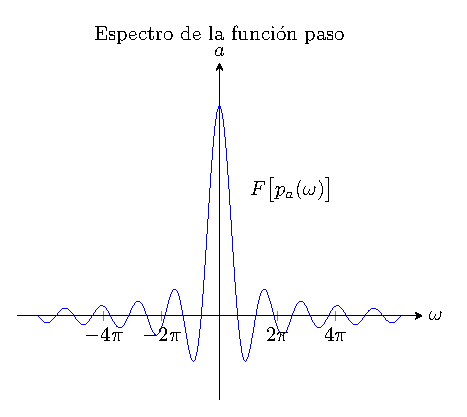
\includegraphics[scale=0.8]{Imagenes/T_Funcionpaso.eps}
    \caption{TF de la función paso rectangular.}
    \label{fig:figura_Tfuncionpaso}
\end{figure}
\end{frame}
% % \textbf{Problema a cuenta: } Calcula la TF de un pulso triangular, como se muestra en la siguiente figura:
% % \begin{figure}[H]
% %     \centering
% %     \includestandalone{Figuras/Tarea-01-Pulso_Triangular}
% % \end{figure}
% % \begin{align*}
% % f (x) = \begin{cases}
% % h(1 - a \, \abs{x}) & \abs{x} < \dfrac{1}{a} \\
% % 0 & \abs{x} > \dfrac{1}{a}
% % \end{cases}
% % \end{align*}

\subsection*{la ecuación de calor}

\begin{frame}
\frametitle{La ecuación de calor}
La ecuación de calor: la temperatura $u (x, t)$ de una barra semiinfinita está determinada por la EDP:
\pause
\begin{align*}
\pdv{u}{t} = \pdv[2]{u}{x} \hspace{1.5cm} x > 0, t > 0
\end{align*}
\pause
sujeta a la condición inicial:
\pause
\begin{align*}
u (x, 0) = \begin{cases}
1, & 0 < x < 1  \\
0, & x > 1
\end{cases}
\end{align*}
\end{frame}
\begin{frame}
\frametitle{La ecuación de calor}
Y la CDF $u (0, t) = 0$, ver la figura (\ref{fig:figura_plot_Ejemplo_06_01}).
\end{frame}
\begin{frame}
\frametitle{La ecuación de calor}
\begin{figure}[H]
  \centering
  \includegraphics[scale=0.7]{Imagenes/Plot_Ejemplo_06_01.pdf}
  \caption{Estado inicial de la barra.}
  \label{fig:figura_plot_Ejemplo_06_01}
\end{figure}
\end{frame}
\begin{frame}
\frametitle{La ecuación de calor}
\textocolor{red}{Por resolver: }
\\
\bigskip
Determina la temperatura en la barra para cualquier tiempo $t$ y en cualquier distancia $x$ a partir de $x = 0$.
\end{frame}
\begin{frame}
\frametitle{Solución}
Dado que la variable $x$ cambia de $0$ a $\infty$ y como el valor de $u(x, t)$ en $x = 0$ está indicado, \pause podemos tomar la TF seno en ambos lados de la EDP para la variable $x$, que queda excluida de la ecuación transformada.
\end{frame}
\begin{frame}
\frametitle{Solución}
Se tiene entonces que la ecuación dada es:
\pause
\begin{eqnarray*}
\begin{aligned}
&\dv{t} \overline{u}_{s} (\xi, t) = \sqrt{\dfrac{2}{\pi}} \scaleint{6ex}_{\bs 0}^{\infty} \pdv[2]{u}{x} \sin \xi x \dd{x} = \\[0.5em] \pause
&= \sqrt{\dfrac{2}{\pi}} \, \big[ \xi \, u(0, t) \big] - \xi^{2} \, \overline{u}_{s} (\xi, t) = \\[0.5em] \pause
&= - \xi^{2} \, \overline{u}_{s} (x , t)
\end{aligned}
\end{eqnarray*}
\end{frame}
\begin{frame}
\frametitle{Solución}
Por lo que:
\pause
\begin{align}
\overline{u}_{s} (\xi, t) = c \, \exp(-\xi^{2} \, t)
\label{eq:ecuacion_ejemplo_1_27_i}
\end{align}
donde $c$ es una constante arbitraria.
\end{frame}
\begin{frame}
\frametitle{Solución}
Como se tiene la condición inicial:
\pause
\begin{eqnarray*}
\begin{aligned}
u (x, 0) &= \begin{cases}
1, & 0 < x < 1  \\
0, & x > 1
\end{cases}
\\
\therefore \quad \overline{u}_{s} (\xi, 0) &= \sqrt{\dfrac{2}{\pi}} \scaleint{6ex}_{\bs 0}^{\infty} u (x, 0) \sin \xi x \dd{x}=
\end{aligned}
\end{eqnarray*}
\end{frame}
\begin{frame}
\frametitle{Solución}
\begin{eqnarray}
\begin{aligned}[b]
&= \sqrt{\dfrac{2}{\pi}} \scaleint{6ex}_{\bs 0}^{1} \sin \xi x \dd{x} = \\[0.5em] \pause 
&= \sqrt{\dfrac{2}{\pi}} \, \bigg[ \dfrac{- \cos \xi x}{\xi} \bigg] \eval_{0}^{1} = \\[0.5em] \pause
&= \sqrt{\dfrac{2}{\pi}} \, \bigg[ \dfrac{1 - \cos \xi}{\xi} \bigg]
\end{aligned}
\label{eq:ecuacion_ejemplo_1_27_ii}
\end{eqnarray}
\end{frame}
\begin{frame}
\frametitle{Solución}
Por lo que, de las ecs. (\ref{eq:ecuacion_ejemplo_1_27_i}) y (\ref{eq:ecuacion_ejemplo_1_27_ii}), tenemos que:
\pause
\begin{align*}
c = \sqrt{\dfrac{2}{\pi}} \, \bigg[ \dfrac{1 - \cos \xi}{\xi} \bigg]
\end{align*}
\end{frame}
\begin{frame}
\frametitle{Solución}  
Ocupando este valor de $c$ en la ec. (\ref{eq:ecuacion_ejemplo_1_27_i}), se llega a:
\pause
\begin{align*}
u (x, t) = \dfrac{2}{\pi} \scaleint{6ex}_{\bs 0}^{\infty} \dfrac{1 - \cos \xi}{\xi} \, \exp(-\xi^{2} t) \, \sin \xi x\dd{\xi}
\end{align*}
\pause
Que es la función de temperatur
\end{frame}
\begin{frame}
\frametitle{Solución gráfica}
Que se muestra en la figura 
\end{frame}
\begin{frame}[plain]
\begin{figure}[H]
    \centering
    \includegraphics[scale=0.8]{Imagenes/Plot_Ejemplo_06_02.eps}
    \caption{Distribución de temperaturas en la barra como función de la posición $x$ y del tiempo $t$.}
    \label{fig:figura_plot_Ejemplo_06_02}
\end{figure}
\end{frame}

\subsection*{Ejemplo 9}

\begin{frame}
\frametitle{La ecuación de onda}
Con la TF determina el desplazamiento $y (x, t)$ en una cuerda infinita oscilante, \pause considerando que la cuerda está inicialmente en reposo y que el desplazamiento inicial es $f (x)$ para $-\infty < x < \infty$.
\end{frame}
\begin{frame}
\frametitle{Por resolver}
Demuestra que la solución se presenta de la forma:
\pause
\begin{align*}
y (x, t) = \dfrac{1}{2} \big[ f (x + c \, t) + f (x - c \, t) \big]
\end{align*}
\end{frame}
\begin{frame}
\frametitle{Solución al ejercicio}
La ecuación de onda unidimensional de una cuerda oscilante está dada por:
\pause
\begin{align*}
\pdv[2]{y}{t} = c^{2} \pdv[2]{y}{x}, \hspace{1.5cm} -\infty < x < \infty, \hspace{0.2cm} t > 0
\end{align*}
\end{frame}
\begin{frame}
\frametitle{Solución al ejercicio}
Ya que la variable $x$ cambia de $-\infty$ a $\infty$, para remover la variable de la EDP, \pause ocupamos la TF compleja en la ecuación de onda para obtener:
\pause
\begin{eqnarray*}
\begin{aligned}
\dv[2]{\overline{y}(\xi, t)}{t} &= \dfrac{c^{2}}{\sqrt{2 \pi}} \scaleint{6ex}_{\bs -\infty}^{\infty} \pdv[2]{y(x, t)}{x} \, \exp(i \xi x) \dd{x} = \\[0.5em] \pause
&= - c^{2} \, \xi^{2} \, \overline{y} (\xi, t)
\end{aligned}
\end{eqnarray*}
\end{frame}
\begin{frame}
\frametitle{Solución al ejercicio}
Por lo tanto:
\pause
\begin{align}
\overline{y} (\xi, t) &= A \, \cos (c \, \xi \, t) + B \, \sin (c \, \xi \, t) \label{eq:ecuacion_ejemplo_1_29_i} \\[0.5em]
\overline{y}_{t} (\xi, t) &= A \, c \, \xi \, \sin (c \, \xi \, t) + B \, c \, \xi \, \cos (c \, \xi \, t) \label{eq:ecuacion_ejemplo_1_29_ii}
\end{align}
donde $A$ y $B$ son dos constantes arbitrarias.
\end{frame}
\begin{frame}
\frametitle{Solución al ejercicio}
Ahora, las condiciones iniciales son:
\pause
\begin{align}
y (x, 0) &= \mbox{desplazamiento inicial } = f (x) \label{eq:ecuacion_ejemplo_1_29_iii} \\[0.5em]
\pdv{y}{t} (x, 0) &= 0 \label{eq:ecuacion_ejemplo_1_29_iv}
\end{align}
ya que la velocidad inicial de la cuerda es cero.
\end{frame}
\begin{frame}
\frametitle{Solución al ejercicio}
De las ecs. (\ref{eq:ecuacion_ejemplo_1_29_ii}) y (\ref{eq:ecuacion_ejemplo_1_29_iii}), se tiene que:
\pause
\begin{align}
\overline{y} (\xi, t) &= \dfrac{1}{\sqrt{2 \pi}} \scaleint{6ex}_{\bs -\infty}^{\infty} f (x) \, \exp(i \xi x) \dd{x} = \overline{f} (\xi) \label{eq:ecuacion_ejemplo_1_29_v} \\[0.5em]
\pdv{\overline{y}}{t} (\xi, 0) &= \overline{y}_{t} (\xi, 0) = 0 \label{eq:ecuacion_ejemplo_1_29_vi}
\end{align}
\end{frame}
\begin{frame}
\frametitle{Solución al ejercicio}
De la ec. (\ref{eq:ecuacion_ejemplo_1_29_i}), se tiene que:
\pause
\begin{align}
\overline{y} (\xi, 0) = A = \overline{f} (\xi) \hspace{1.5cm} \mbox{por la ec. (\ref{eq:ecuacion_ejemplo_1_29_v})}
\end{align}
\end{frame}
\begin{frame}
\frametitle{Solución al ejercicio}
También por la ec. (\ref{eq:ecuacion_ejemplo_1_29_ii}), se obtiene:
\pause
\begin{align}
\overline{y}_{t} (\xi, 0) = B \, c \, \xi \hspace{1.5cm} \mbox{por la ec. (\ref{eq:ecuacion_ejemplo_1_29_vi})}
\end{align}
\end{frame}
\begin{frame}
\frametitle{Solución al ejercicio}
Entonces  $B = 0$. Así:
\pause
\begin{align*}
\overline{y}(\xi, t) = \overline{f}(\xi) \, \cos (c \, \xi \, t)
\end{align*}
\end{frame}
\begin{frame}
\frametitle{Solución al ejercicio}
Tomando la transformada inversa de la ecuación anterior, se llega a:
\pause
\begin{eqnarray*}
\begin{aligned}
&y (x, t) = \dfrac{1}{\sqrt{2 \pi}} \scaleint{6ex}_{\bs \infty}^{+ \infty} \bigg[ \dfrac{\exp(i c \xi t) + \exp(-i c \xi t)}{2} \bigg] \times \\[0.5em]
&\times  \exp(-i \, \xi \, x) \dd{\xi} = 
\end{aligned}
\end{eqnarray*}
\end{frame}
\begin{frame}
\frametitle{Solución al ejercicio}
\begin{eqnarray*}
\begin{aligned}
&= \dfrac{1}{2} \, \dfrac{1}{\sqrt{2 \pi}} \scaleint{6ex}_{\bs \infty}^{+ \infty} \overline{f} (\xi) \cdot \bigg[ \exp(-i \xi (x {-} c t)) + \\[0.5em]
&+ \exp(-i \xi (x {+} c t)) \bigg] \dd{\xi} =
\end{aligned}
\end{eqnarray*}
\end{frame}
\begin{frame}
\frametitle{Solución al ejercicio}
\begin{eqnarray*}
\begin{aligned}
&= \dfrac{1}{2} \bigg[ \dfrac{1}{\sqrt{2 \pi}} \scaleint{6ex}_{-\infty}^{+\infty} \overline{f} (\xi) \, \exp(- \xi (x - c t)) \dd{\xi} + \\[0.5em]
&+ \dfrac{1}{2} \dfrac{1}{\sqrt{2 \pi}} \scaleint{6ex}_{-\infty}^{+\infty} \overline{f} (\xi) \cdot \exp(- \xi (x + c t)) \dd{\xi} \bigg] \\[0.5em] \pause
&\Rightarrow \hspace{0.3cm} y(x, t) = \dfrac{1}{2} \big[ f (x -c t) + f (x +  ct) \big]
\end{aligned}
\end{eqnarray*}
\end{frame}

\section{Ejercicios a cuenta}
\frame{\tableofcontents[currentsection, hideothersubsections]}
\subsection{Inciso 1}

% \noindent
% %Ref. Patra Example 1.5
\begin{frame}
\frametitle{Primer enunciado}
Calcula la TF de:
\begin{align*}
f (x) = \begin{cases}
1 - x^{2}, & \abs{x} \leq 1 \\
0, & \abs{x} > 1
\end{cases}
\end{align*}
\end{frame}
\begin{frame}
\frametitle{Primer enunciado}
Y con ese resultado, evalúa la siguiente integral:
\begin{align*}
\scaleint{6ex}_{\bs0}^{\infty} \dfrac{x \, \cos x - \sin x}{x^{3}} \, \cos \dfrac{x}{2} \dd{x}
\end{align*}
\end{frame}

\subsection{Inciso 2}
% %Ref. Patra Example 1.12

\begin{frame}
\frametitle{Segundo enunciado}
Con las siguientes funciones:
\begin{align*}
g (x) = e^{-a x} \hspace{2cm} f (x) \begin{cases}
1, & 0 < x < a \\
0, & x > a
\end{cases} 
\end{align*}
y con la relación de Parseval pertinente:
\end{frame}
\begin{frame}
\frametitle{Segundo enunciado}
Demuestra que:
\begin{align*}
\scaleint{6ex}_{\bs 0}^{\infty} \dfrac{\sin a t}{t (a^{2} + t^{2})} \dd{t} = \dfrac{\pi}{2} \, \dfrac{1 - \exp(-a^{2})}{a^{2}}
\end{align*}
\end{frame}
% \\[0.5em]
% \noindent
% %Ref. Patra Example 1.38
% \textbf{Ejercicio a cuenta (59). } La temperatura $u(x, t)$ en una barra semiinfinita $0 \leq x < \infty$ satisface la siguiente EDP:
% \begin{align*}
% \pdv{u}{t} =\kappa \, \pdv[2]{u}{x}
% \end{align*}
% sujeta a las siguientes condiciones:
% \begin{align*}
% u(x, 0) &= 0, \hspace{0.5cm} x \geq 0 \\[0.5em]
% \pdv{u}{x} &= - \lambda \hspace{0.5cm} \mbox{una constante, cuando \quad} x = 0, \hspace{0.2cm} t > 0  
% \end{align*}
% Calcula la temperatura para valores $x > 0$ y $t > 0$.

\end{document}